% trimer_bsse.tex — Chapter 4: Trimer BSSE Analysis — BSSE Results
% Project: rmrresearch/bsse_db | Branch: fcuantico
% Molecules: H2O (complete), Ne (complete), HF (complete)

% ======================================================================
\section{\ce{H2O} Trimer BSSE Results}
% ======================================================================

% ----------------------------------------------------------------------
\subsection{Total BSSE vs O--O Distance}
% ----------------------------------------------------------------------

Figure~\ref{fig:h2o_trimer_plot1} shows the total BSSE as a function
of O--O distance $R$ for all three levels of theory.

\begin{figure}[!ht]
    \centering
    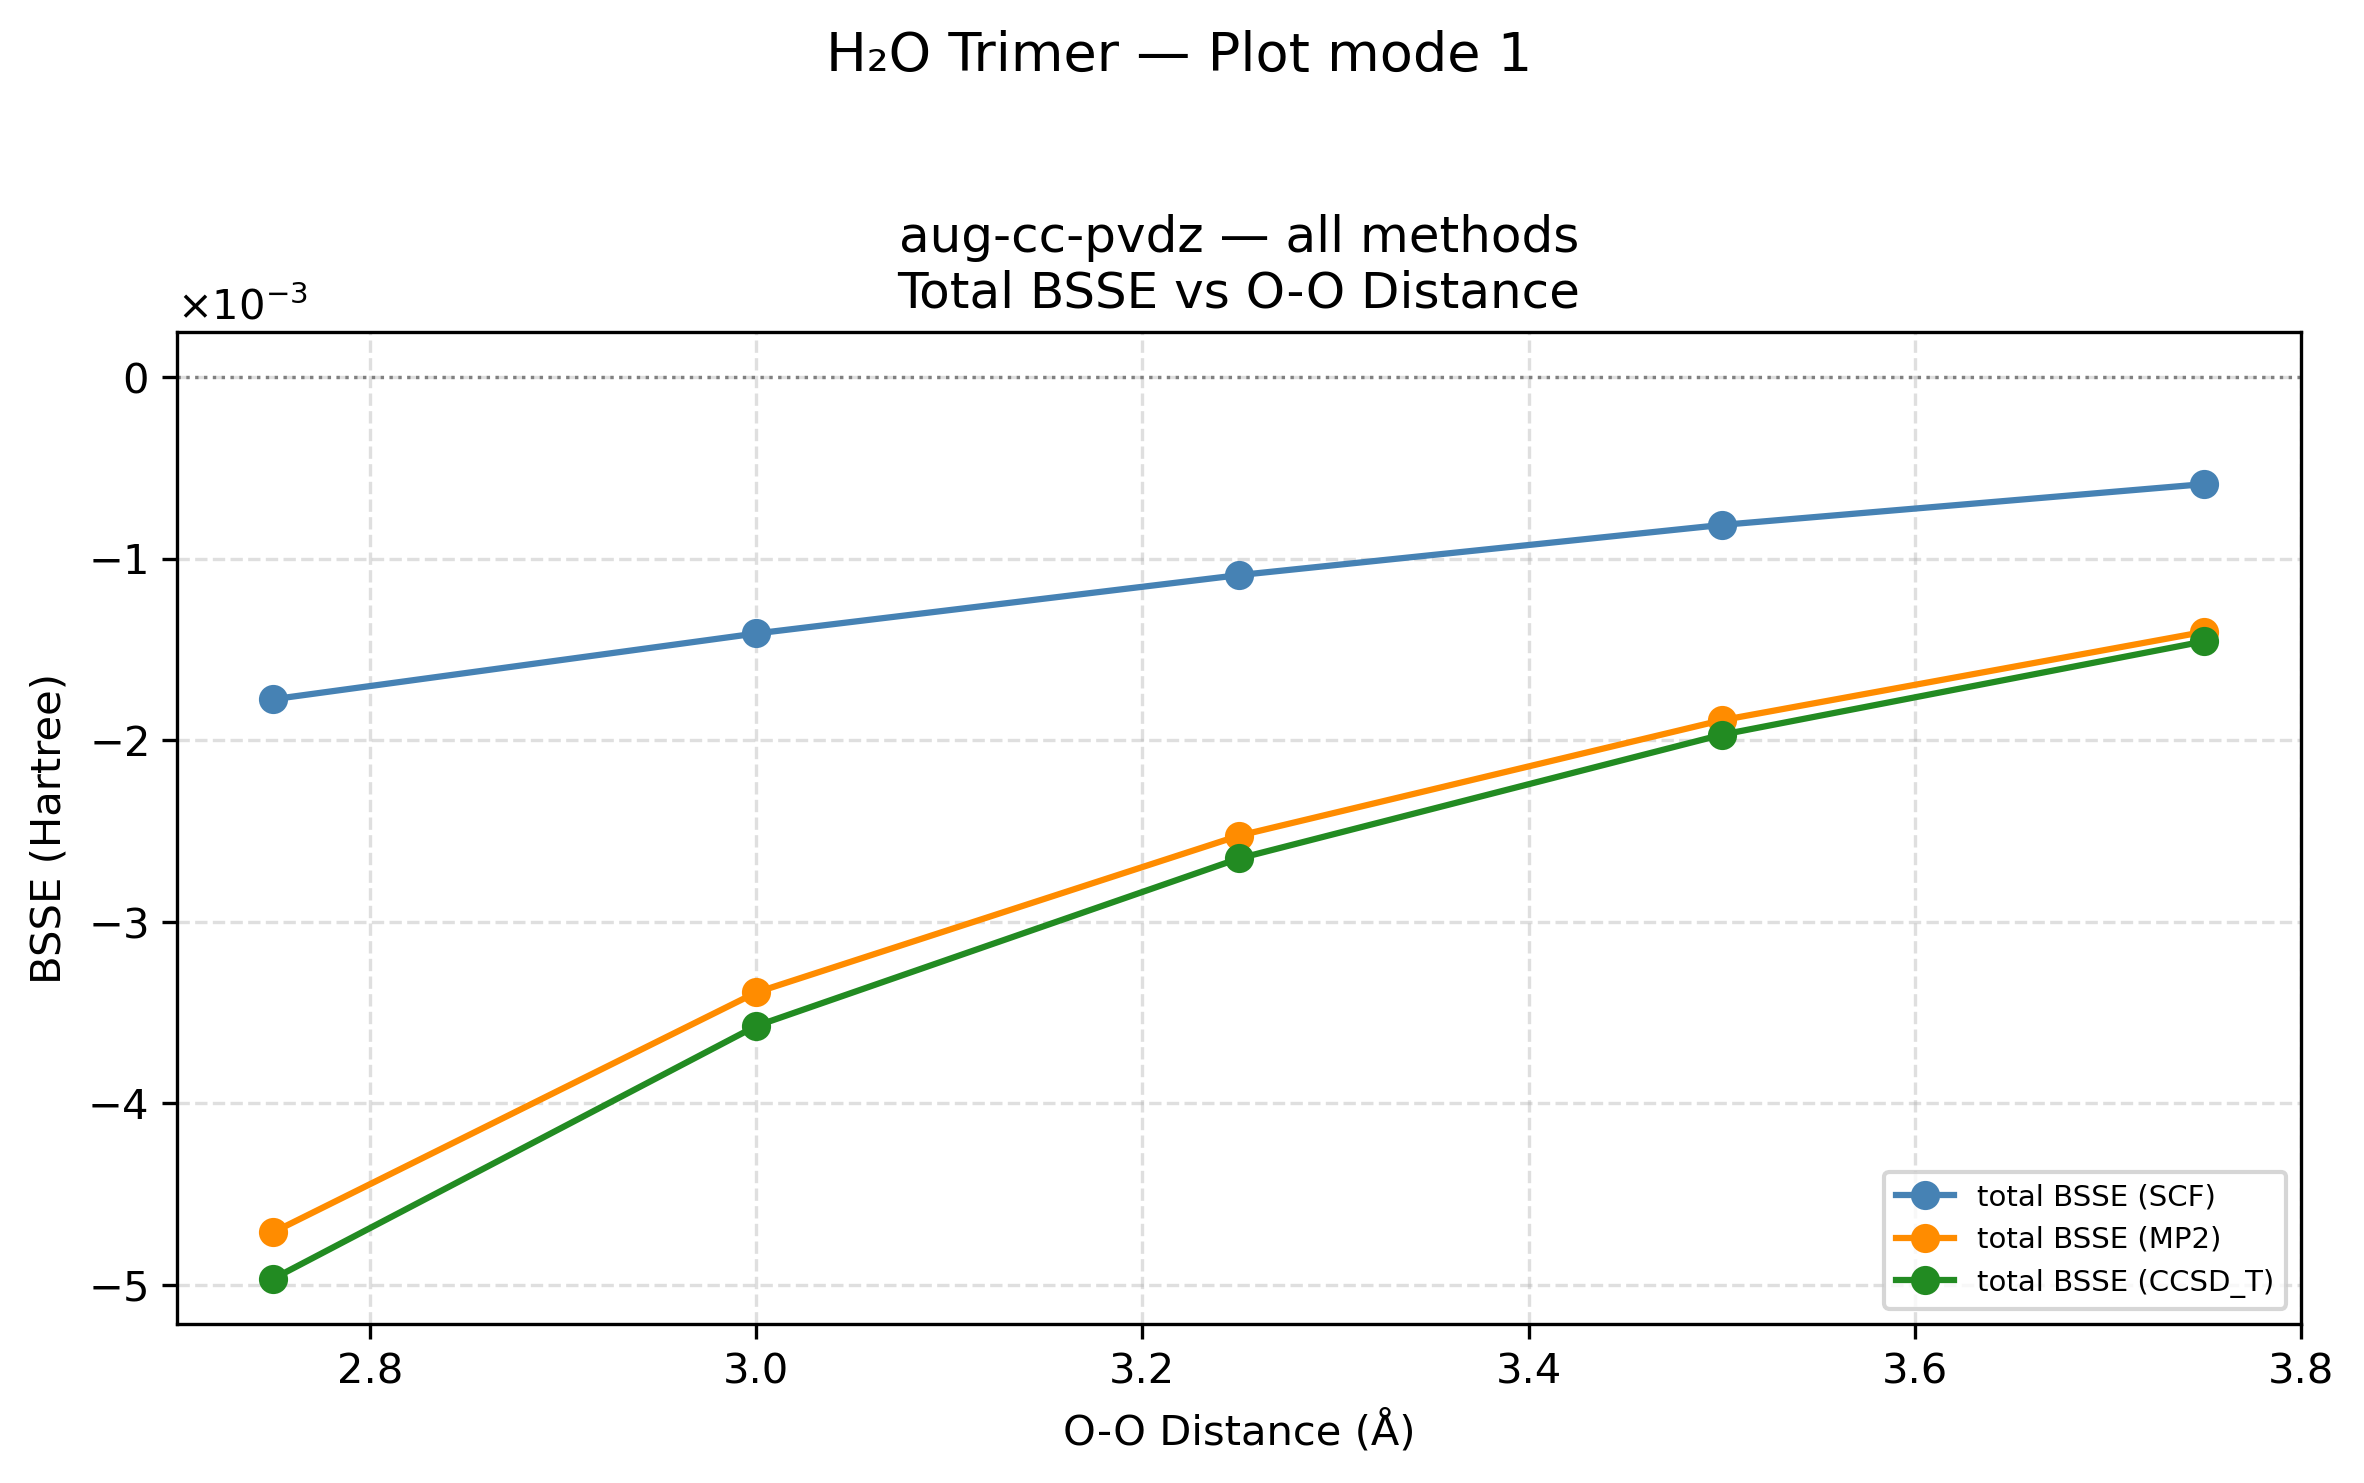
\includegraphics[width=1.0\textwidth]{figures/trimer/H2O_trimer/plot1_all_aug-cc-pvdz.png}
    \caption{Total BSSE vs O--O distance $R$ for the \ce{H2O} trimer
    at the aug-cc-pVDZ level. Blue circles: SCF; orange squares: MP2;
    green triangles: CCSD(T). All values are in Hartree. All three
    curves approach zero monotonically with increasing $R$. The MP2
    and CCSD(T) curves are close in magnitude and significantly larger
    than the SCF contribution at all distances sampled.}
    \label{fig:h2o_trimer_plot1}
\end{figure}

All three curves are negative and approach zero monotonically with
increasing $R$, consistent with the expected reduction of basis set
overlap at larger separations. At the shortest distance ($R = \SI{2.75}{\angstrom}$) the
total BSSE values are approximately $-1.8 \times 10^{-3}$~Ha (SCF),
$-4.7 \times 10^{-3}$~Ha (MP2), and $-5.0 \times 10^{-3}$~Ha
(CCSD(T)). The MP2 and CCSD(T) curves are close throughout the range,
while the SCF contribution is smaller in magnitude by roughly a factor
of three.

% ----------------------------------------------------------------------
\subsection{Two-Body and Three-Body Decomposition}
% ----------------------------------------------------------------------

Figure~\ref{fig:h2o_trimer_plot2} separates the total BSSE into its
two-body ($\theta^{(2)}$) and three-body ($\theta^{(3)}$) components
for each level of theory.

\begin{figure}[!ht]
    \centering
    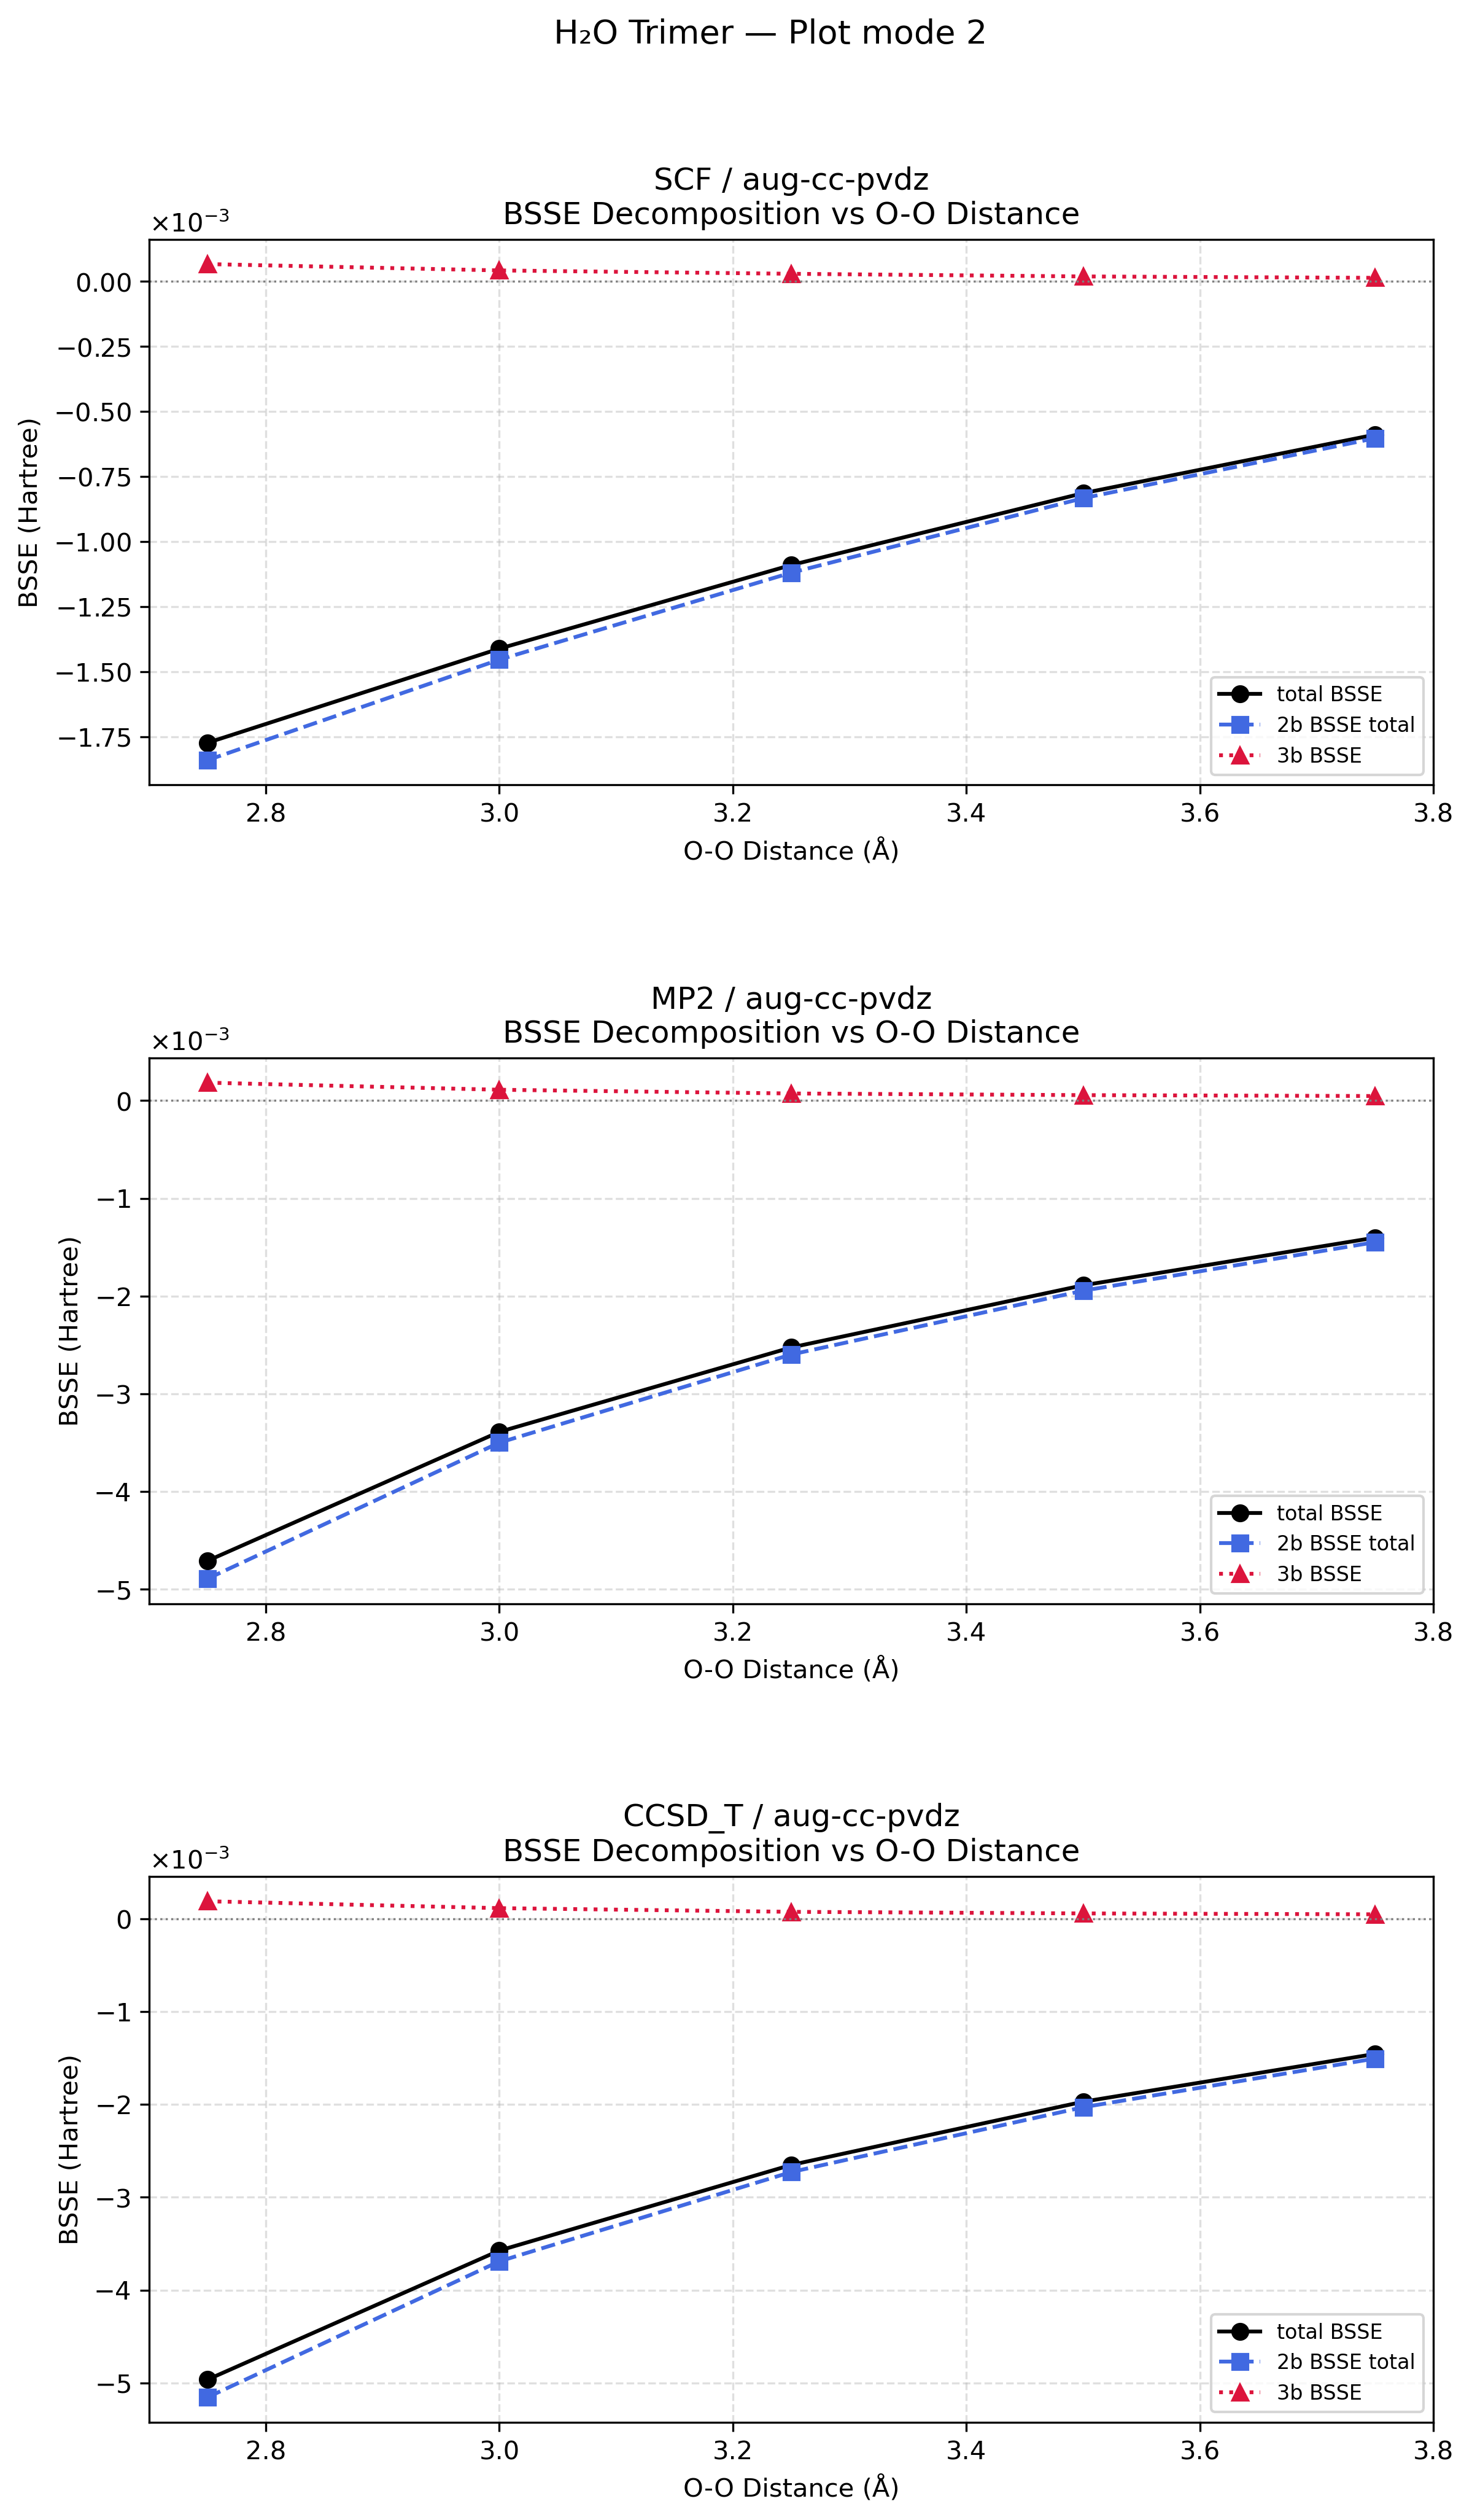
\includegraphics[width=0.7\textwidth]{figures/trimer/H2O_trimer/plot2_all_aug-cc-pvdz.png}
    \caption{BSSE body-order decomposition vs O--O distance $R$ for the
    \ce{H2O} trimer at the aug-cc-pVDZ level. Each panel corresponds to
    one level of theory (SCF, MP2, CCSD(T)). Black circles: total BSSE;
    blue dashed: 2-body total ($\theta^{(2)}$); red triangles: 3-body
    term ($\theta^{(3)}$). The total and 2-body curves are nearly
    indistinguishable in all three panels. The 3-body term is positive
    and remains close to zero across the full range of $R$.}
    \label{fig:h2o_trimer_plot2}
\end{figure}

In all three panels the total BSSE and the 2-body total are nearly
indistinguishable, indicating that the 2-body term accounts for
essentially all of the BSSE. The 3-body contribution $\theta^{(3)}$
is positive in sign (opposite to the 2-body term) and remains close
to zero across the full range of $R$ and all three methods. The
dominance of the 2-body term is consistent across SCF, MP2, and
CCSD(T).

% ----------------------------------------------------------------------
\subsection{Per-Pair Two-Body BSSE}
% ----------------------------------------------------------------------

Figure~\ref{fig:h2o_trimer_plot3} resolves the 2-body BSSE into
contributions from each of the three monomer pairs: AB, AC, and BC.

\begin{figure}[!ht]
    \centering
    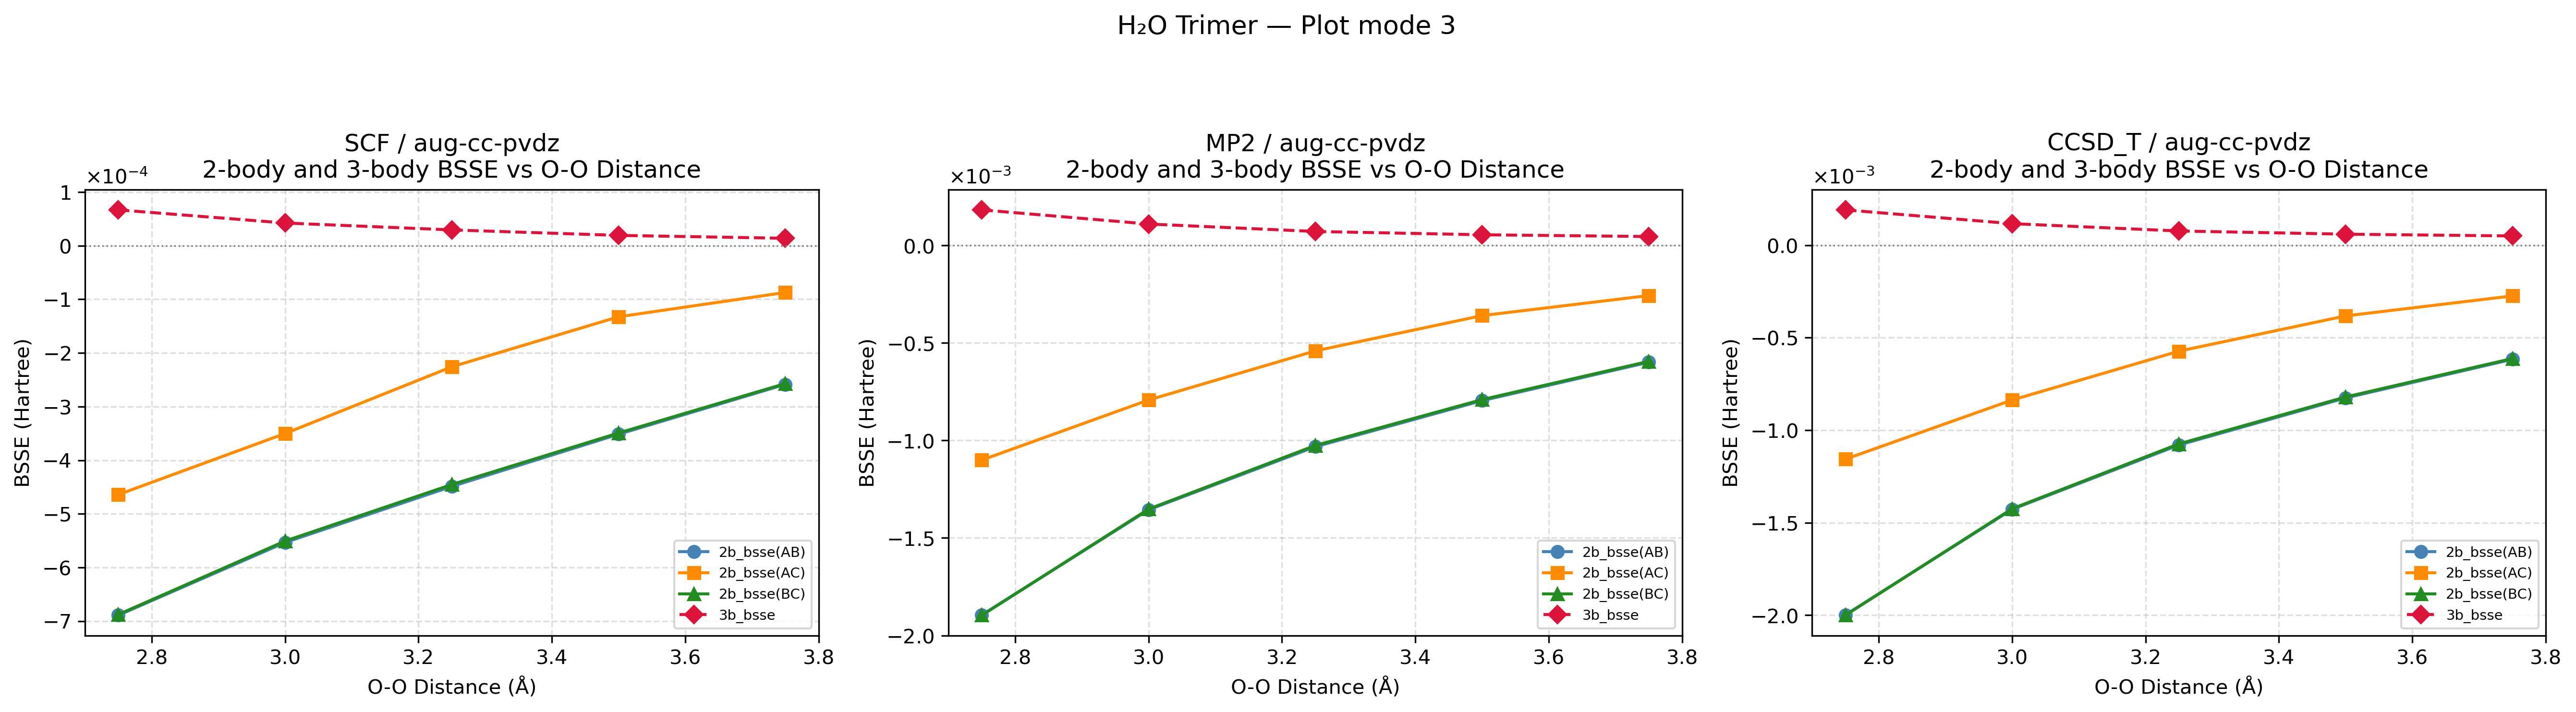
\includegraphics[width=0.7\textwidth]{figures/trimer/H2O_trimer/plot3_all_aug-cc-pvdz.png}
    \caption{Per-pair 2-body and 3-body BSSE vs O--O distance $R$ for
    the \ce{H2O} trimer at the aug-cc-pVDZ level. Each panel
    corresponds to one level of theory. Note the difference in $y$-axis
    scale between the SCF panel ($\times 10^{-4}$~Ha) and the MP2 and
    CCSD(T) panels ($\times 10^{-3}$~Ha). Blue circles: $\theta^{(2)}$(AB);
    orange squares: $\theta^{(2)}$(AC); green triangles: $\theta^{(2)}$(BC);
    red dashed diamonds: $\theta^{(3)}$. The AB and BC pair contributions
    are nearly equal across all methods and distances. The AC pair
    contribution is consistently smaller in magnitude than AB and BC.}
    \label{fig:h2o_trimer_plot3}
\end{figure}

The AB and BC pair contributions are nearly equal at all $R$ values
and across all three methods, while the AC pair contribution is
consistently smaller in magnitude --- approximately half the value of
AB and BC at $R = \SI{3.25}{\angstrom}$ (CCSD(T)). The 3-body term
$\theta^{(3)}$ is positive and small relative to all three pair
contributions.

% TODO: pending PI discussion — physical interpretation of AC pair asymmetry.
% The AC pair has a different relative orientation compared to AB and BC
% in the equilateral triangle geometry (O-O facing geometry), which may
% explain the consistently smaller 2b_bsse(AC). Whether this is due to
% the specific monomer orientation or a more general geometric effect
% requires PI confirmation before asserting in the text.

\clearpage

% ----------------------------------------------------------------------
\subsection{Two-Body BSSE Decomposition at $R = \SI{3.25}{\angstrom}$}
% ----------------------------------------------------------------------

Figure~\ref{fig:h2o_trimer_plot4} shows the FORM~II decomposition of
the 2-body BSSE at the representative configuration $R =
\SI{3.25}{\angstrom}$ (configuration~2) at the CCSD(T) level. Each
pair contribution $\theta^{(2)}(IJ)$ is broken down into its two
monomer-in-dimer-basis $\delta$ terms.

\begin{figure}[!ht]
    \centering
    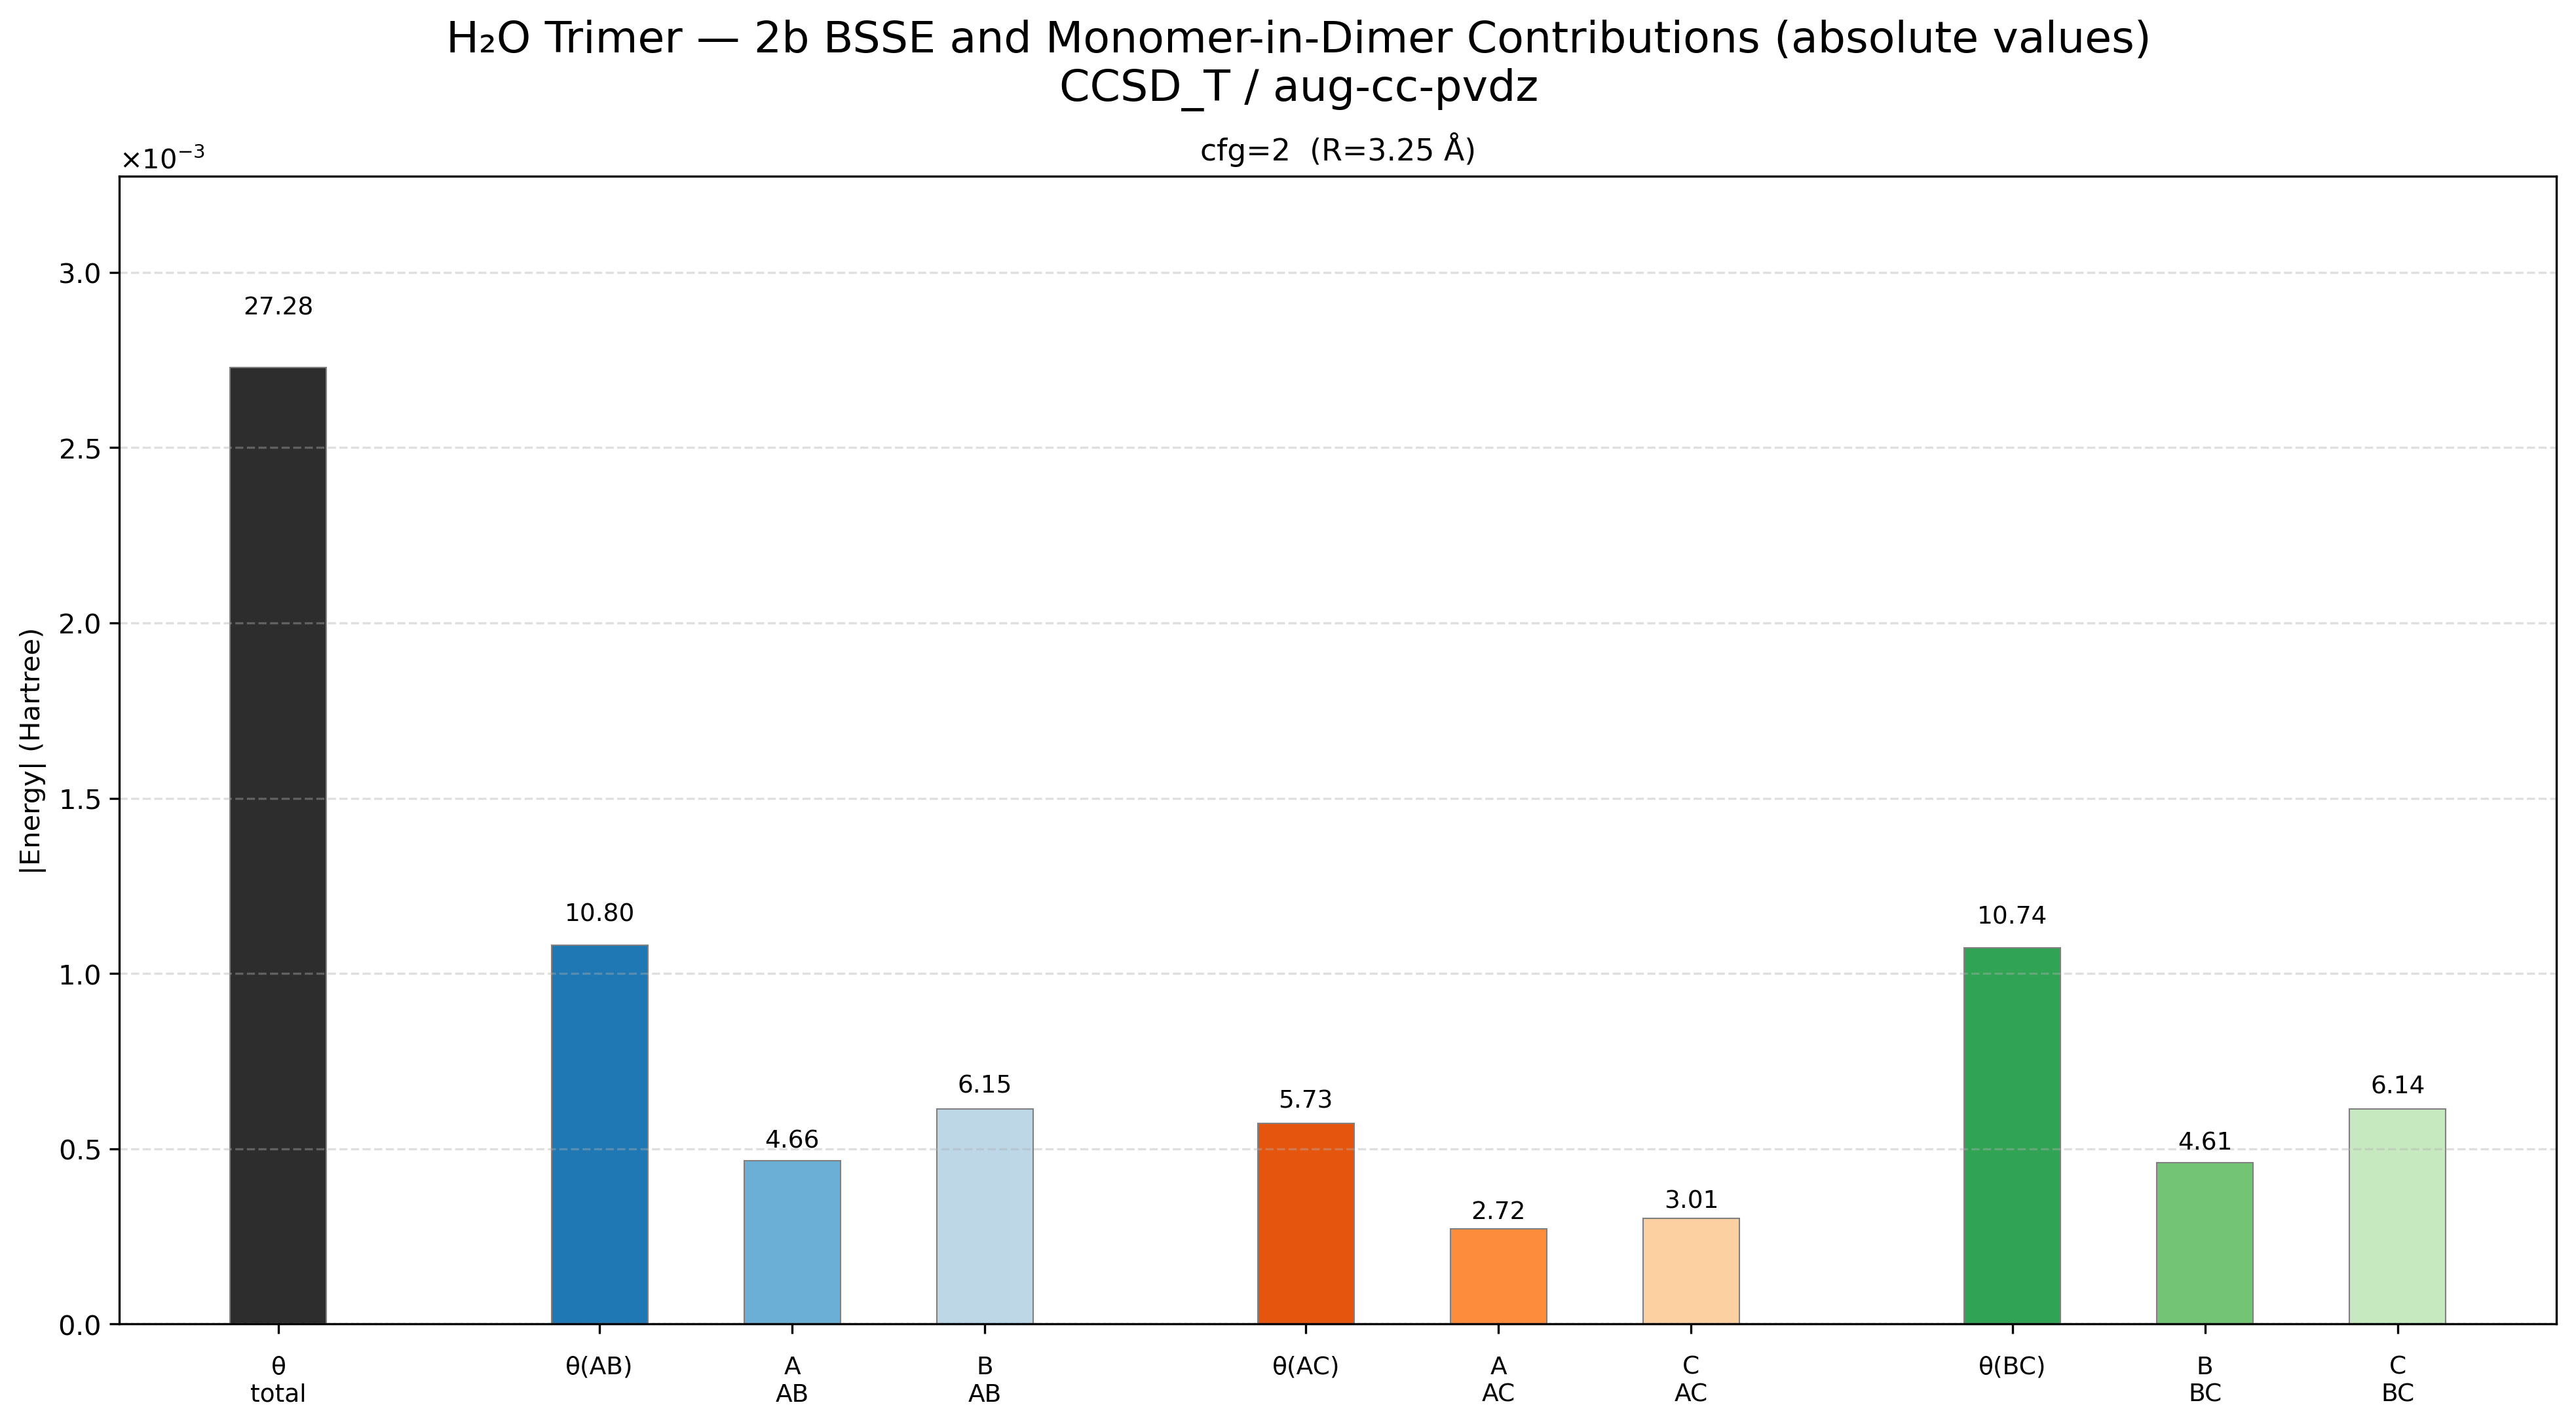
\includegraphics[width=1.0\textwidth]{figures/trimer/H2O_trimer/plot4_CCSD_T_aug-cc-pvdz_part3.png}
    \caption{FORM~II decomposition of the 2-body BSSE for the \ce{H2O}
    trimer at $R = \SI{3.25}{\angstrom}$ (configuration~2), CCSD(T)/aug-cc-pVDZ.
    All values are absolute values in units of $10^{-3}$~Ha. Black bar:
    total 2-body BSSE $|\theta^{(2)}|= 27.28 \times 10^{-3}$~Ha. Dark
    blue and light blue bars: monomer-in-dimer-basis contributions for
    the AB pair ($|\delta(\text{A in AB})| = 4.66$,
    $|\delta(\text{B in AB})| = 6.15$). Orange and light orange bars:
    AC pair contributions ($|\delta(\text{A in AC})| = 2.72$,
    $|\delta(\text{C in AC})| = 3.01$). Dark green and light green bars:
    BC pair contributions ($|\delta(\text{B in BC})| = 4.61$,
    $|\delta(\text{C in BC})| = 6.14$). The AB and BC pairs are
    comparable in magnitude; the AC pair contributions are approximately
    half those of AB and BC.}
    \label{fig:h2o_trimer_plot4}
\end{figure}

At $R = \SI{3.25}{\angstrom}$ the pair totals are $|\theta^{(2)}(\text{AB})| =
10.80 \times 10^{-3}$~Ha, $|\theta^{(2)}(\text{BC})| = 10.74 \times
10^{-3}$~Ha, and $|\theta^{(2)}(\text{AC})| = 5.73 \times 10^{-3}$~Ha.
Within each pair the two monomer-in-dimer-basis contributions are of
comparable magnitude. The same pattern --- AB $\approx$ BC $>$ AC ---
holds across all five configurations and all three levels of theory.

% ----------------------------------------------------------------------
\subsection{Three-Body BSSE Decomposition at $R = \SI{3.25}{\angstrom}$}
% ----------------------------------------------------------------------

Figure~\ref{fig:h2o_trimer_plot5} shows the FORM~II decomposition of
the 3-body BSSE at the same representative configuration.

\begin{figure}[!ht]
    \centering
    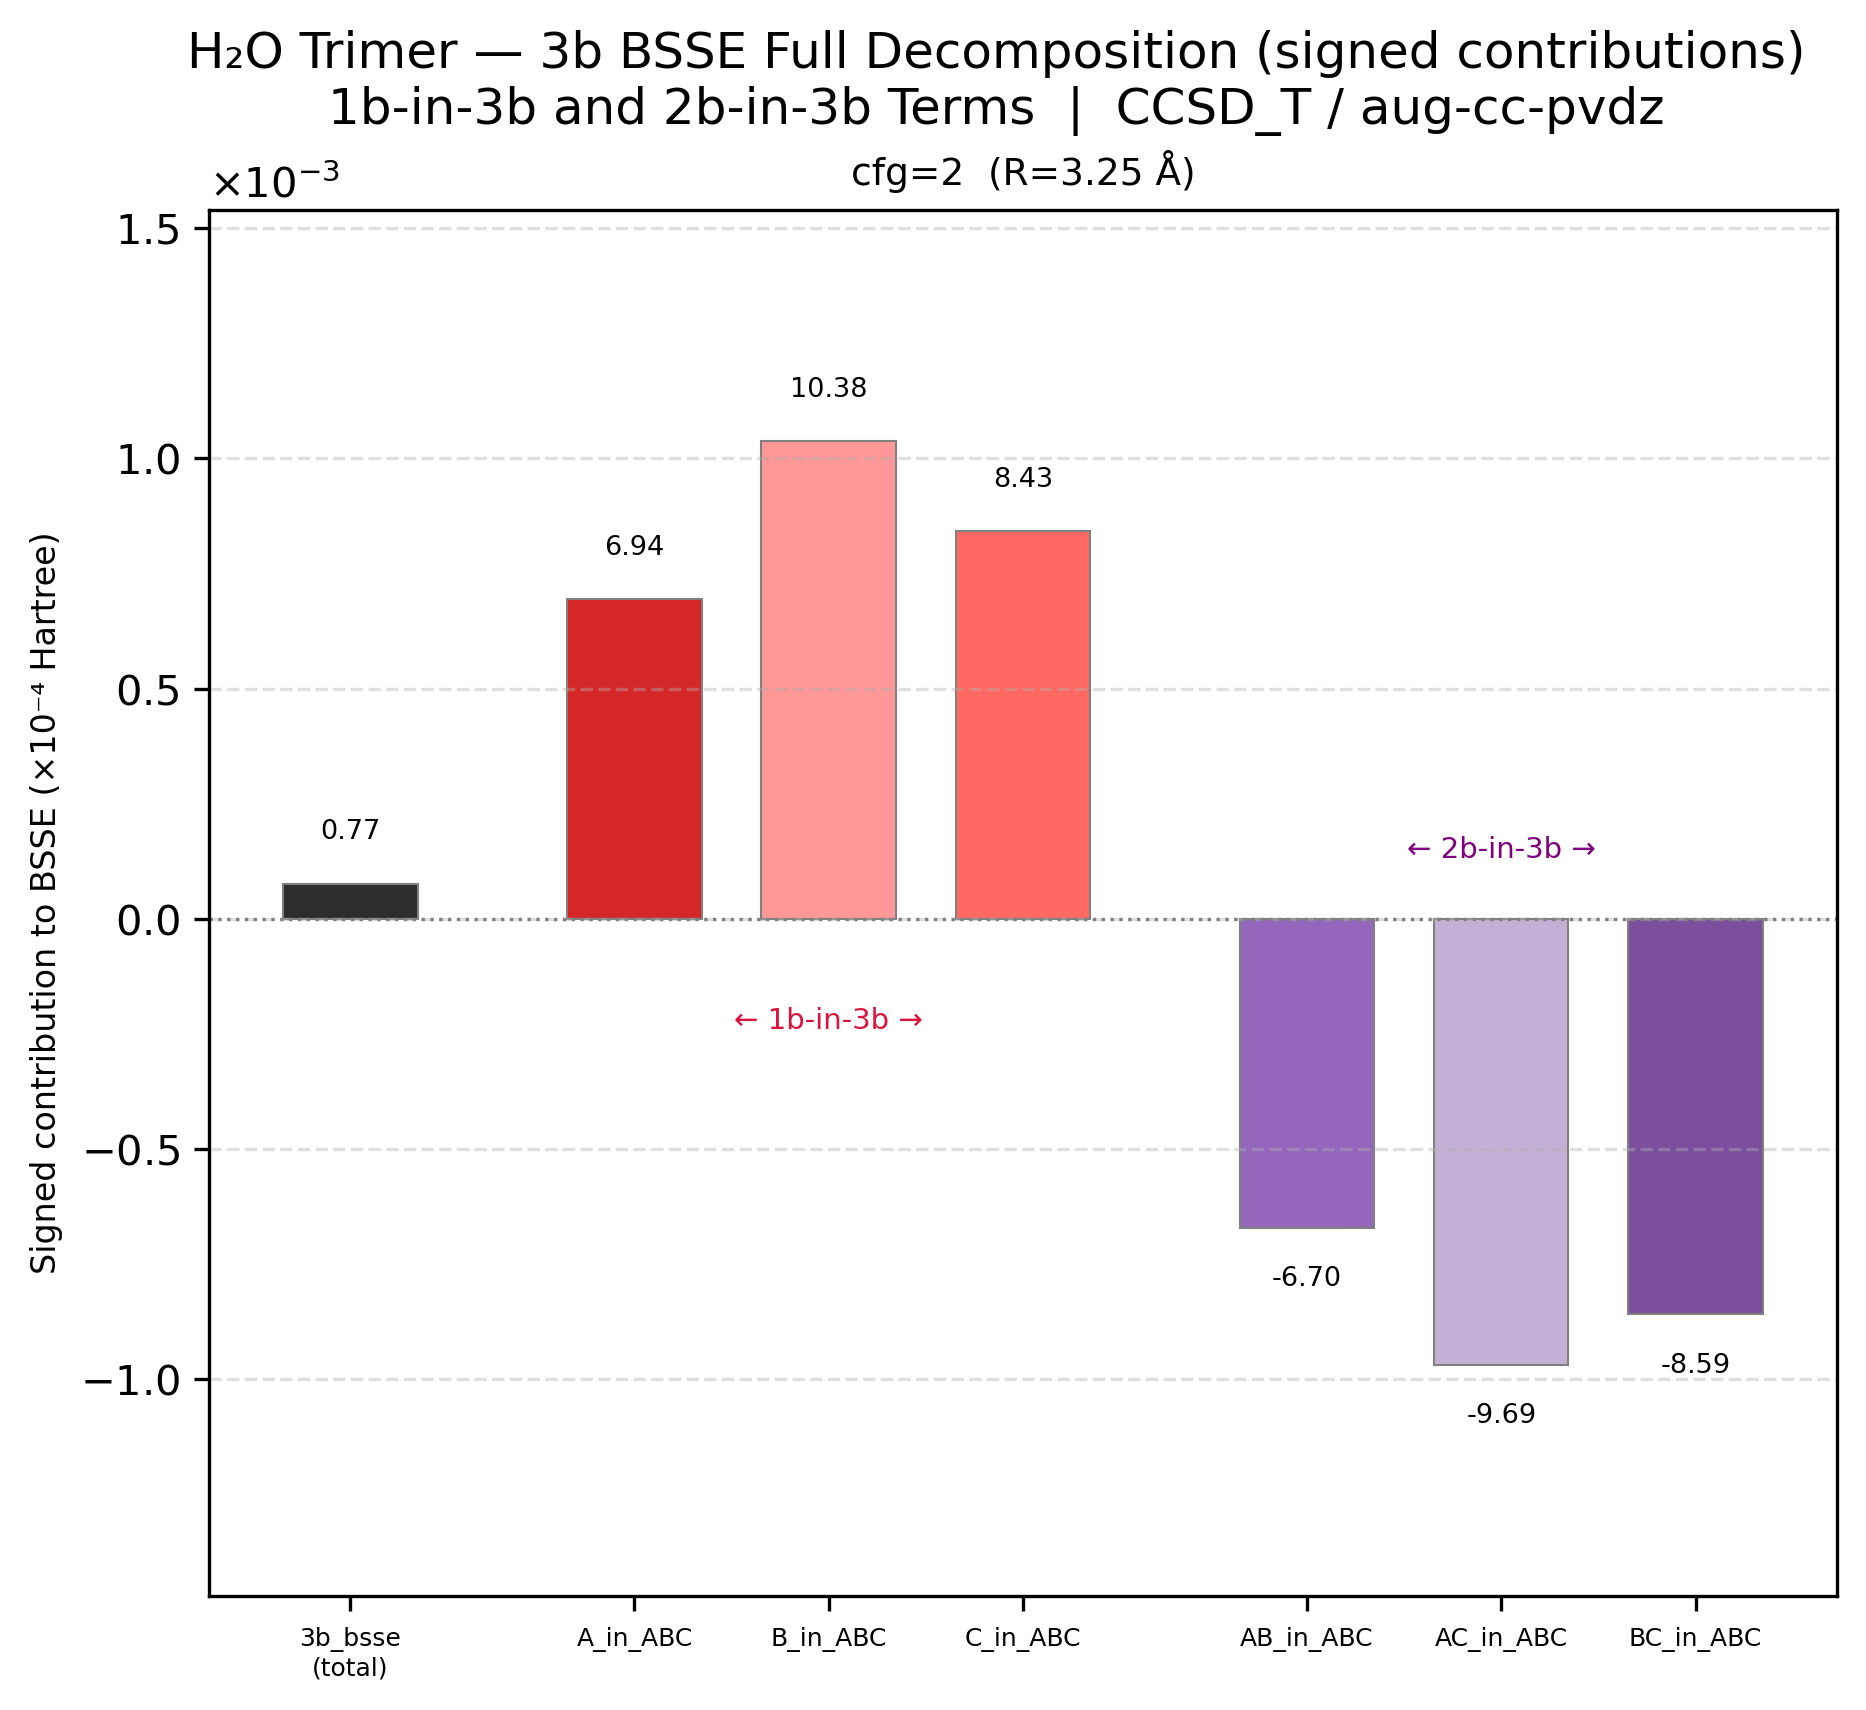
\includegraphics[width=1.0\textwidth]{figures/trimer/H2O_trimer/plot5_CCSD_T_aug-cc-pvdz_part3.png}
    \caption{FORM~II decomposition of the 3-body BSSE for the \ce{H2O}
    trimer at $R = \SI{3.25}{\angstrom}$ (configuration~2),
    CCSD(T)/aug-cc-pVDZ. Signed contributions in units of $10^{-4}$~Ha.
    Black bar: total $\theta^{(3)} = +0.77 \times 10^{-4}$~Ha. Red bars
    (positive): 1b-in-3b terms
    $\delta(\text{A in ABC}) = +6.94$,
    $\delta(\text{B in ABC}) = +10.38$,
    $\delta(\text{C in ABC}) = +8.43$.
    Purple bars (negative): 2b-in-3b terms
    $\delta(\text{AB in ABC}) = -6.70$,
    $\delta(\text{AC in ABC}) = -9.69$,
    $\delta(\text{BC in ABC}) = -8.59$.
    The two groups are opposite in sign and nearly equal in magnitude,
    resulting in a small positive net $\theta^{(3)}$.}
    \label{fig:h2o_trimer_plot5}
\end{figure}

\clearpage

The 3-body BSSE $\theta^{(3)}$ is the result of a near-cancellation
between two groups of opposite sign: the 1b-in-3b terms (positive)
and the 2b-in-3b terms (negative). At $R = \SI{3.25}{\angstrom}$ the
net value is $+0.77 \times 10^{-4}$~Ha, approximately one order of
magnitude smaller than the total 2-body BSSE. This near-cancellation
pattern is consistent across all five configurations.

% ----------------------------------------------------------------------
\subsection{Key Findings}
% ----------------------------------------------------------------------

\begin{finding_box}
\textbf{The 2-body term dominates the \ce{H2O} trimer BSSE.}
Across all five O--O distances and all three levels of theory, the
total BSSE is accounted for almost entirely by the sum of the three
pairwise 2-body contributions. The 3-body term $\theta^{(3)}$ is
positive in sign and approximately one order of magnitude smaller than
the 2-body total at all configurations sampled.
\end{finding_box}

\begin{finding_box}
\textbf{The AC pair contributes less 2-body BSSE than AB or BC.}
The per-pair decomposition shows that $\theta^{(2)}(\text{AB}) \approx
\theta^{(2)}(\text{BC})$ across all configurations and methods, while
$\theta^{(2)}(\text{AC})$ is consistently smaller --- approximately
half the AB and BC values at mid-range distances. The 3-body BSSE
arises from a near-cancellation between the 1b-in-3b (positive) and
2b-in-3b (negative) FORM~II delta terms.
\end{finding_box}

\clearpage

% ======================================================================
\section{Ne Trimer BSSE Results}
% ======================================================================

% ----------------------------------------------------------------------
\subsection{Total BSSE vs Ne--Ne Distance}
% ----------------------------------------------------------------------

Figure~\ref{fig:ne_trimer_plot1} shows the total BSSE as a function of
Ne--Ne distance $R$ for all three levels of theory.

\begin{figure}[!ht]
    \centering
    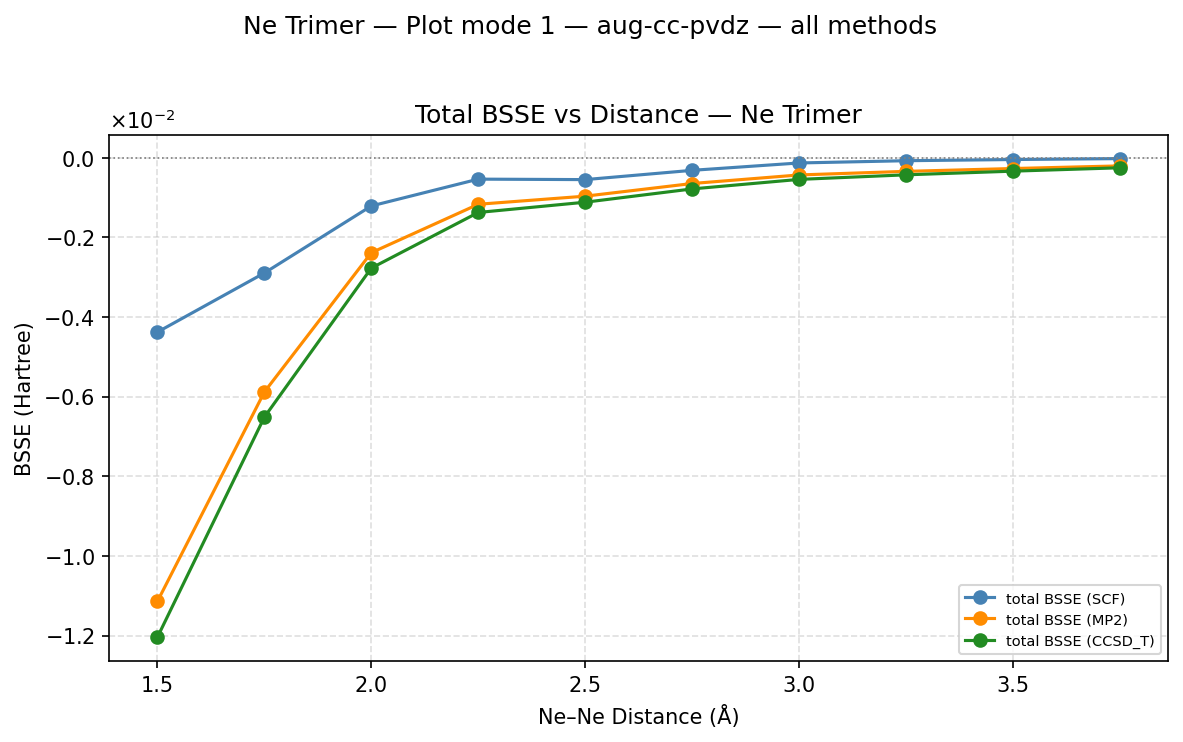
\includegraphics[width=1.0\textwidth]{figures/trimer/Ne_trimer/plot1_Ne_all_aug-cc-pvdz.png}
    \caption{Total BSSE vs Ne--Ne distance $R$ for the Ne trimer at
    the aug-cc-pVDZ level. Blue circles: SCF; orange squares: MP2;
    green triangles: CCSD(T). All values are in Hartree. All three
    curves approach zero monotonically with increasing $R$. At the
    shortest distance ($R = \SI{1.5}{\angstrom}$) the total BSSE
    reaches approximately $-4.5 \times 10^{-3}$~Ha (SCF),
    $-1.1 \times 10^{-2}$~Ha (MP2), and $-1.2 \times 10^{-2}$~Ha
    (CCSD(T)). The MP2 and CCSD(T) curves are close throughout
    the range, while the SCF contribution is smaller in magnitude
    by approximately a factor of three at short range.}
    \label{fig:ne_trimer_plot1}
\end{figure}

All three curves are negative and approach zero monotonically with
increasing $R$, consistent with the reduction of basis set overlap at
larger separations. The BSSE magnitude drops sharply between $R =
\SI{1.5}{\angstrom}$ and $R = \SI{2.0}{\angstrom}$, then decreases
more gradually at longer range. The MP2 and CCSD(T) values are
substantially larger in magnitude than the SCF contribution across the
full range, reflecting the additional basis set incompleteness
introduced by the correlation treatment.

% ----------------------------------------------------------------------
\subsection{Two-Body and Three-Body Decomposition}
% ----------------------------------------------------------------------

Figure~\ref{fig:ne_trimer_plot2} separates the total BSSE into its
two-body ($\theta^{(2)}$) and three-body ($\theta^{(3)}$) components
for each level of theory.

\begin{figure}[!ht]
    \centering
    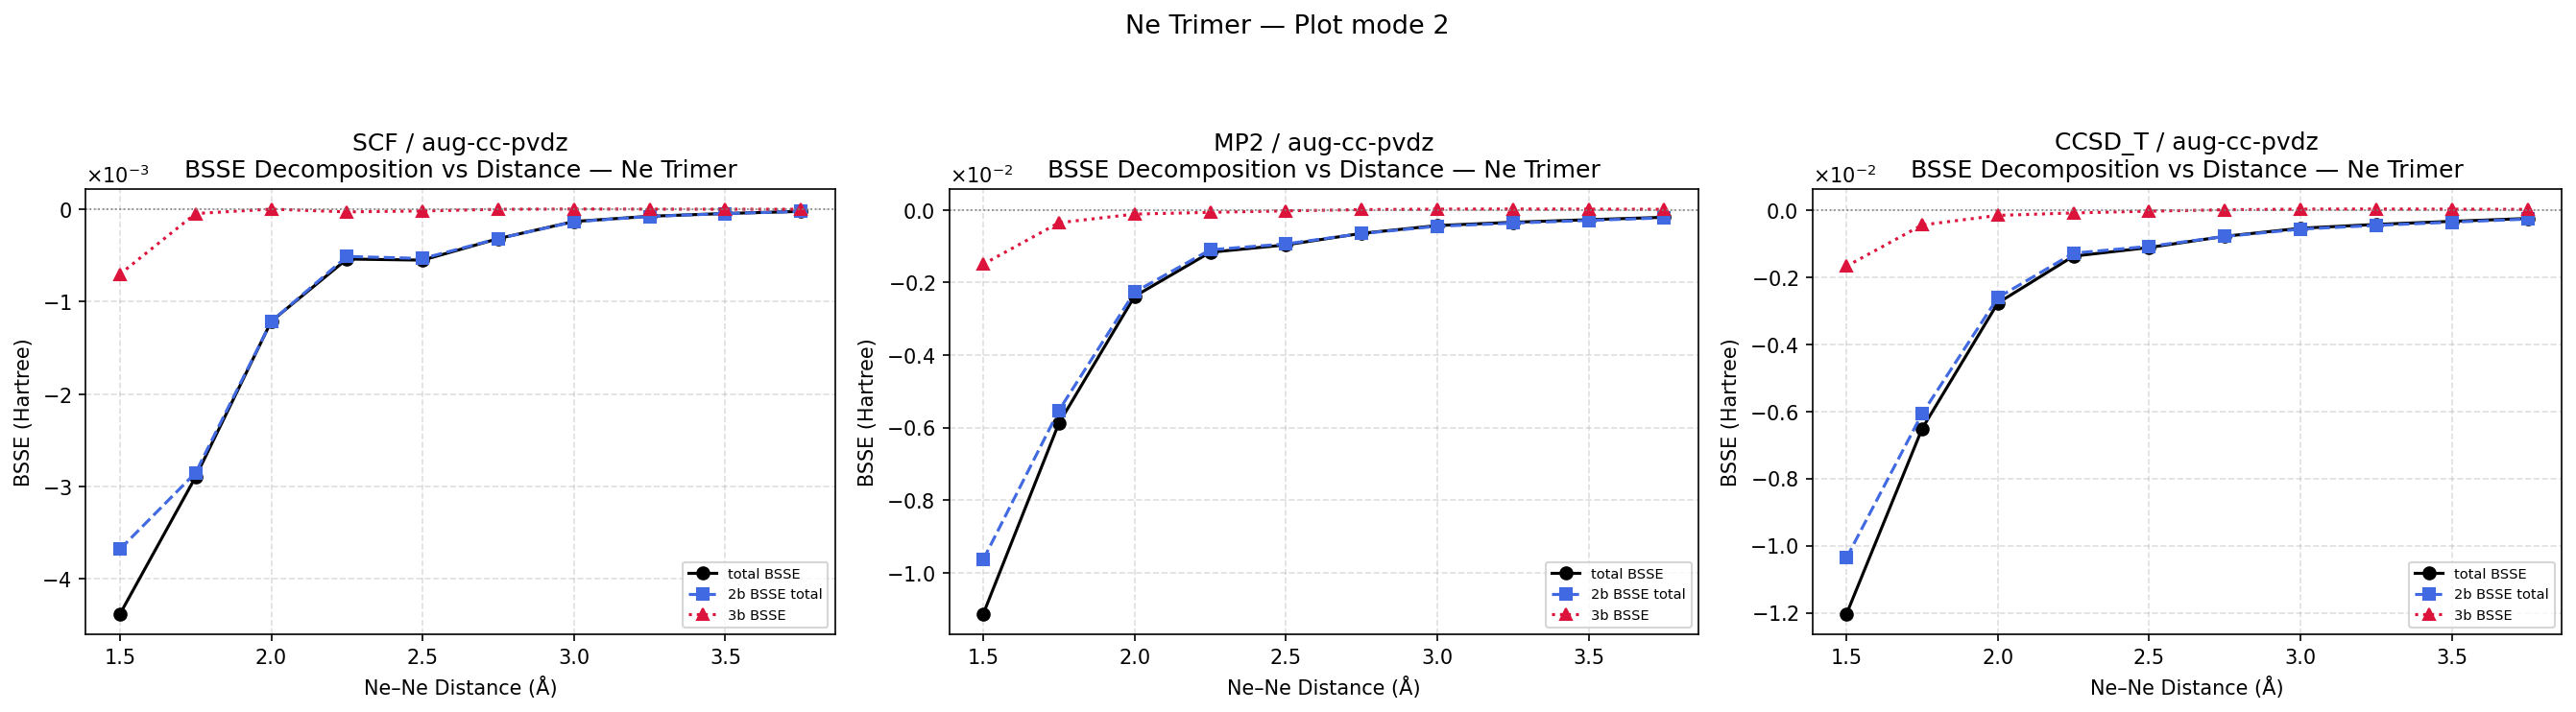
\includegraphics[width=0.7\textwidth]{figures/trimer/Ne_trimer/plot2_Ne_all_aug-cc-pvdz.png}
    \caption{BSSE body-order decomposition vs Ne--Ne distance $R$ for
    the Ne trimer at the aug-cc-pVDZ level. Each panel corresponds to
    one level of theory (SCF, MP2, CCSD(T)). Black circles: total
    BSSE; blue dashed squares: 2-body total ($\theta^{(2)}$); red
    dashed triangles: 3-body term ($\theta^{(3)}$). The total and
    2-body curves are nearly indistinguishable in all three panels.
    At all three levels of theory the 3-body term is negative at short
    range and changes sign to positive with increasing $R$, crossing
    zero near $R = \SI{2.75}{\angstrom}$.}
    \label{fig:ne_trimer_plot2}
\end{figure}

In all three panels the total BSSE and the 2-body total are nearly
indistinguishable, confirming that the 2-body term accounts for
essentially all of the BSSE. The 3-body contribution $\theta^{(3)}$
is small in magnitude relative to the 2-body total at all distances.
A notable feature present at all three levels of theory is a sign
change in $\theta^{(3)}$: the term is negative at short range (where
orbital overlap is significant) and becomes positive at longer range,
crossing zero near $R = \SI{2.75}{\angstrom}$.

% ----------------------------------------------------------------------
\subsection{Per-Pair Two-Body BSSE}
% ----------------------------------------------------------------------

Figure~\ref{fig:ne_trimer_plot3} resolves the 2-body BSSE into
contributions from each of the three monomer pairs: AB, AC, and BC.

\begin{figure}[!ht]
    \centering
    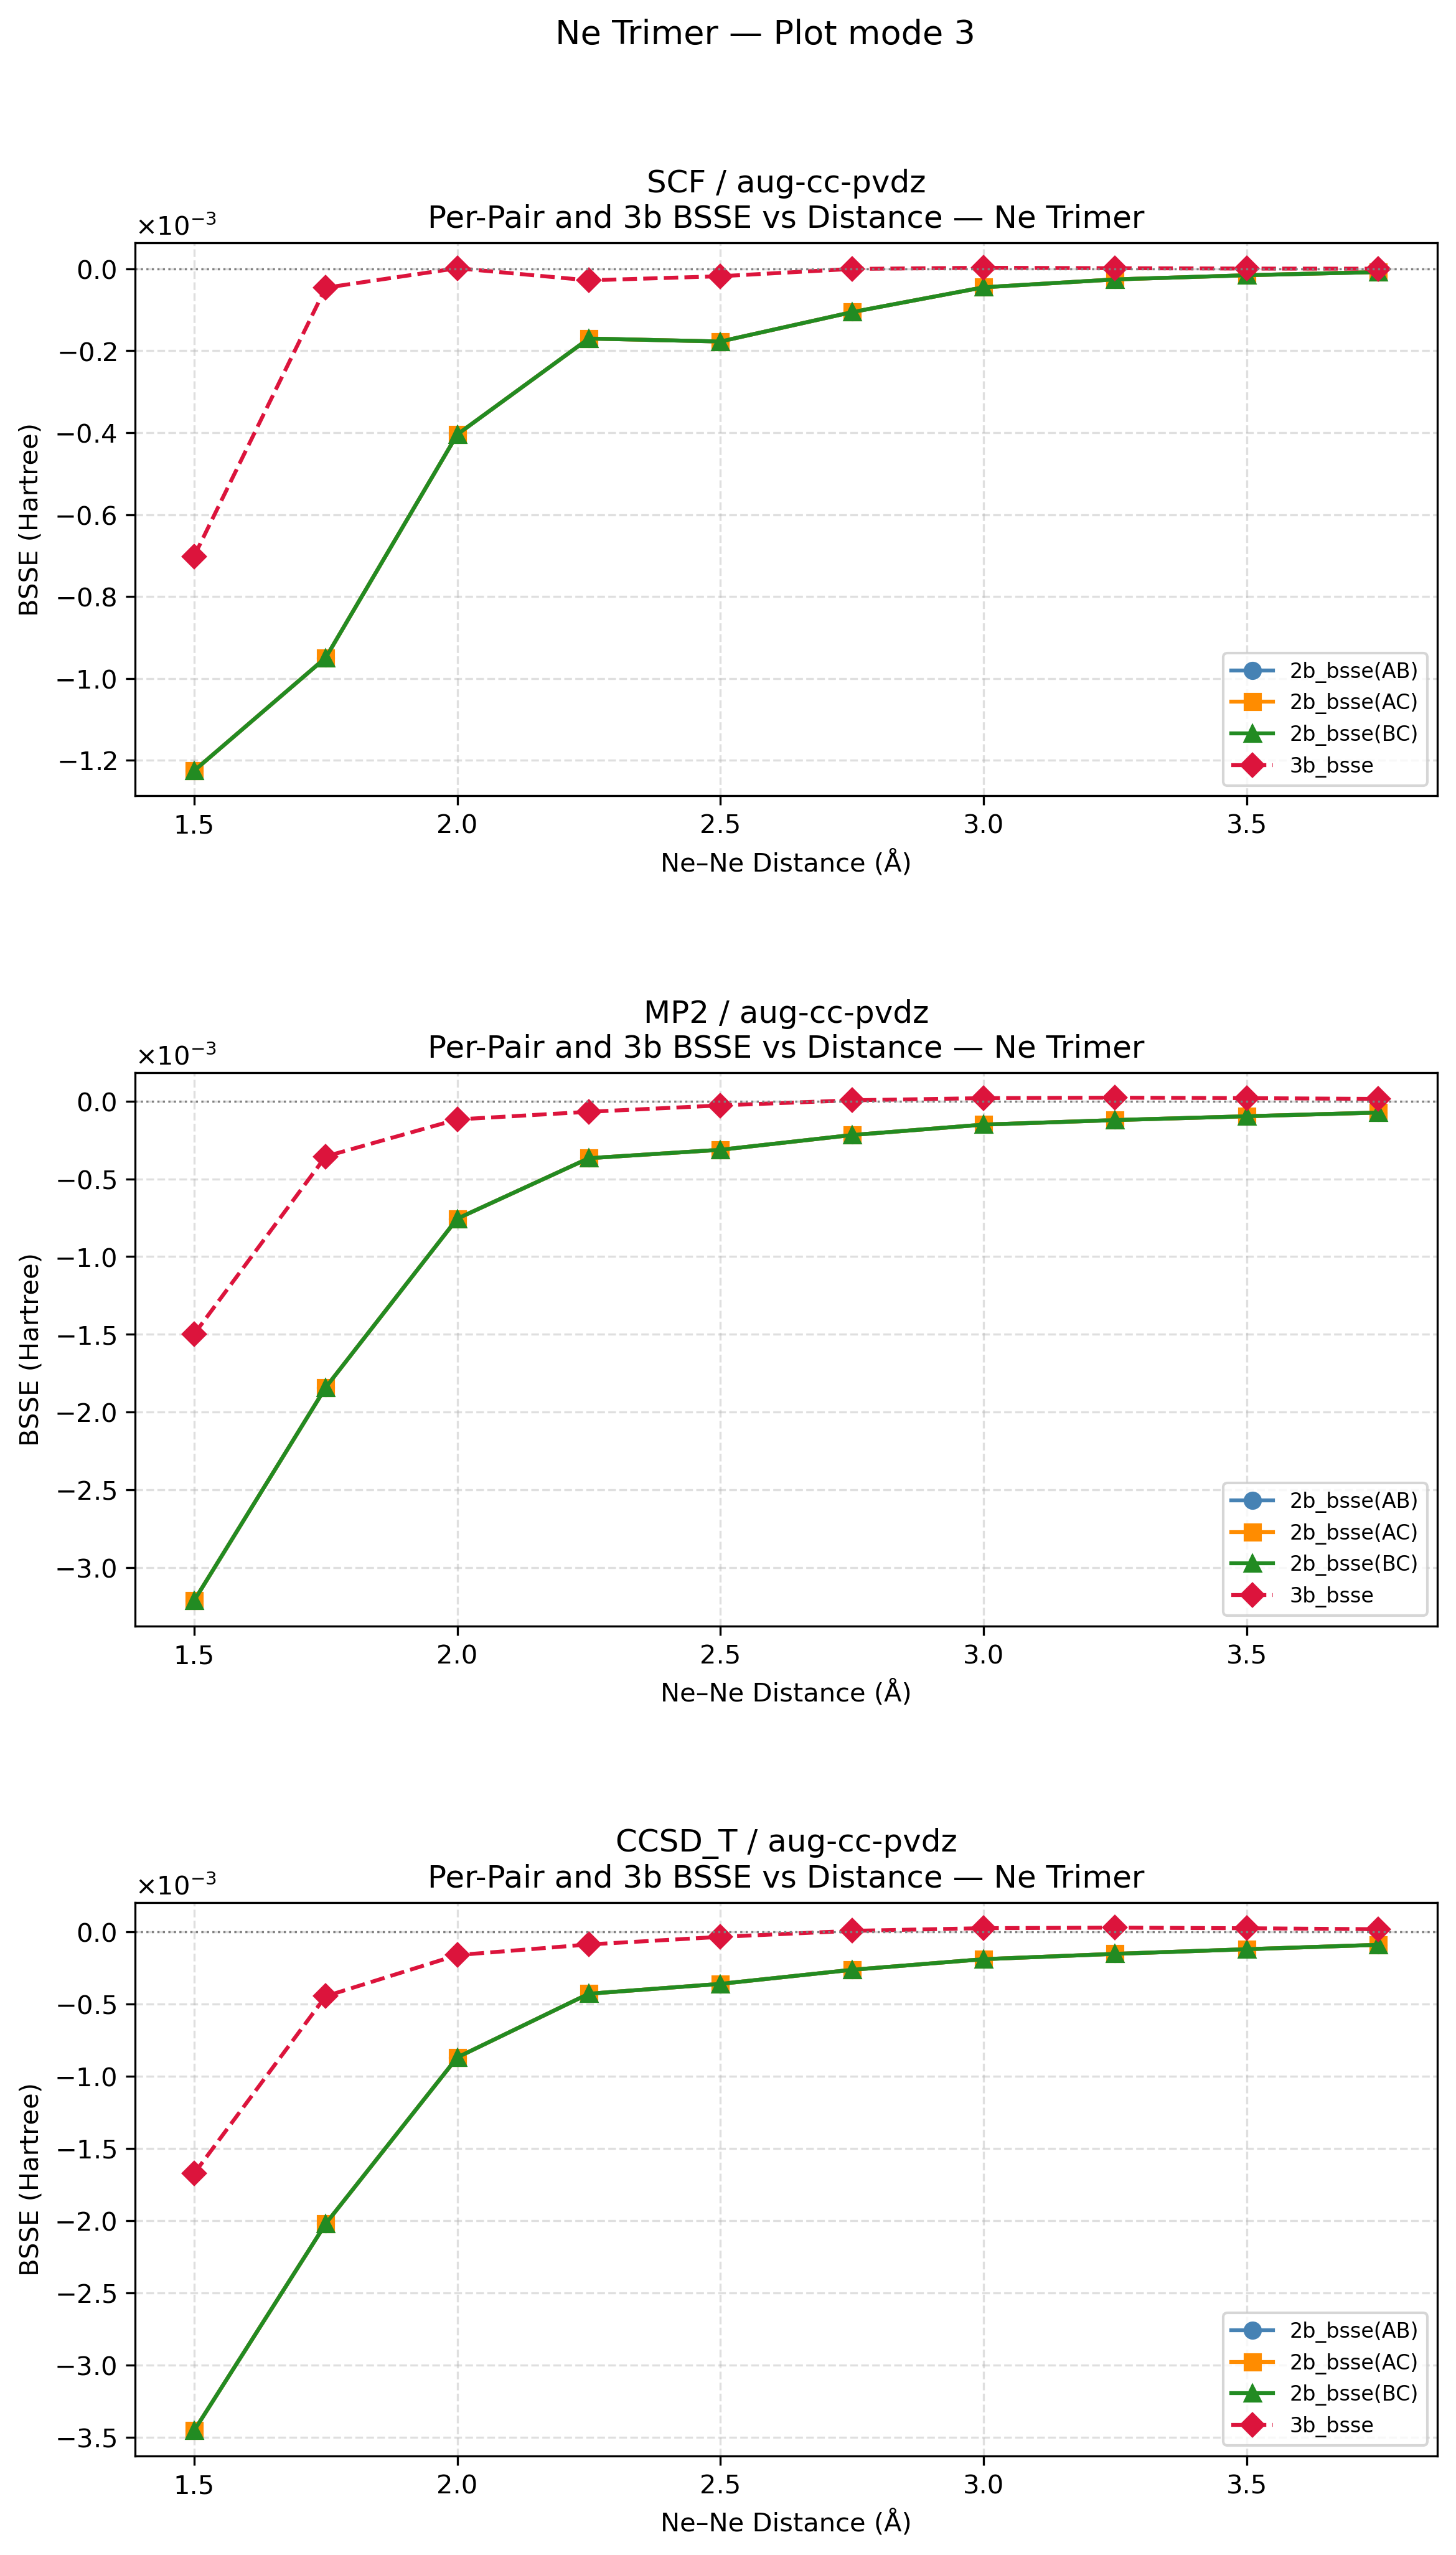
\includegraphics[width=0.7\textwidth]{figures/trimer/Ne_trimer/plot3_Ne_all_aug-cc-pvdz.png}
    \caption{Per-pair 2-body and 3-body BSSE vs Ne--Ne distance $R$
    for the Ne trimer at the aug-cc-pVDZ level. Each panel corresponds
    to one level of theory. Blue circles: $\theta^{(2)}$(AB); orange
    squares: $\theta^{(2)}$(AC); green triangles: $\theta^{(2)}$(BC);
    red dashed diamonds: $\theta^{(3)}$. The three pair contributions
    are exactly equal at every distance and every level of theory,
    reflecting the perfect equilateral symmetry of the Ne trimer:
    $\theta^{(2)}(\text{AB}) = \theta^{(2)}(\text{AC}) =
    \theta^{(2)}(\text{BC})$ at all $R$.}
    \label{fig:ne_trimer_plot3}
\end{figure}

The three pair contributions $\theta^{(2)}(\text{AB})$,
$\theta^{(2)}(\text{AC})$, and $\theta^{(2)}(\text{BC})$ are
numerically identical at every configuration and every level of
theory. In Figure~\ref{fig:ne_trimer_plot3} the three symbols lie
exactly on top of one another, reducing to a single visible curve.
This perfect degeneracy is a direct consequence of the equilateral
triangle geometry and the identity of the Ne monomers: all three
pairs are related by the $C_{3v}$ symmetry of the cluster. In
contrast to the \ce{H2O} trimer, where the AC pair showed a
consistently distinct BSSE from AB and BC, the Ne trimer exhibits
no such pair inequivalence.

\clearpage

% ----------------------------------------------------------------------
\subsection{Two-Body BSSE Decomposition at $R = \SI{2.5}{\angstrom}$}
% ----------------------------------------------------------------------

Figure~\ref{fig:ne_trimer_plot4} shows the FORM~II decomposition of
the 2-body BSSE at the representative configuration $R =
\SI{2.5}{\angstrom}$ (configuration~4) at the CCSD(T) level. Each
pair contribution $\theta^{(2)}(IJ)$ is broken down into its two
monomer-in-dimer-basis $\delta$ terms.

\begin{figure}[!ht]
    \centering
    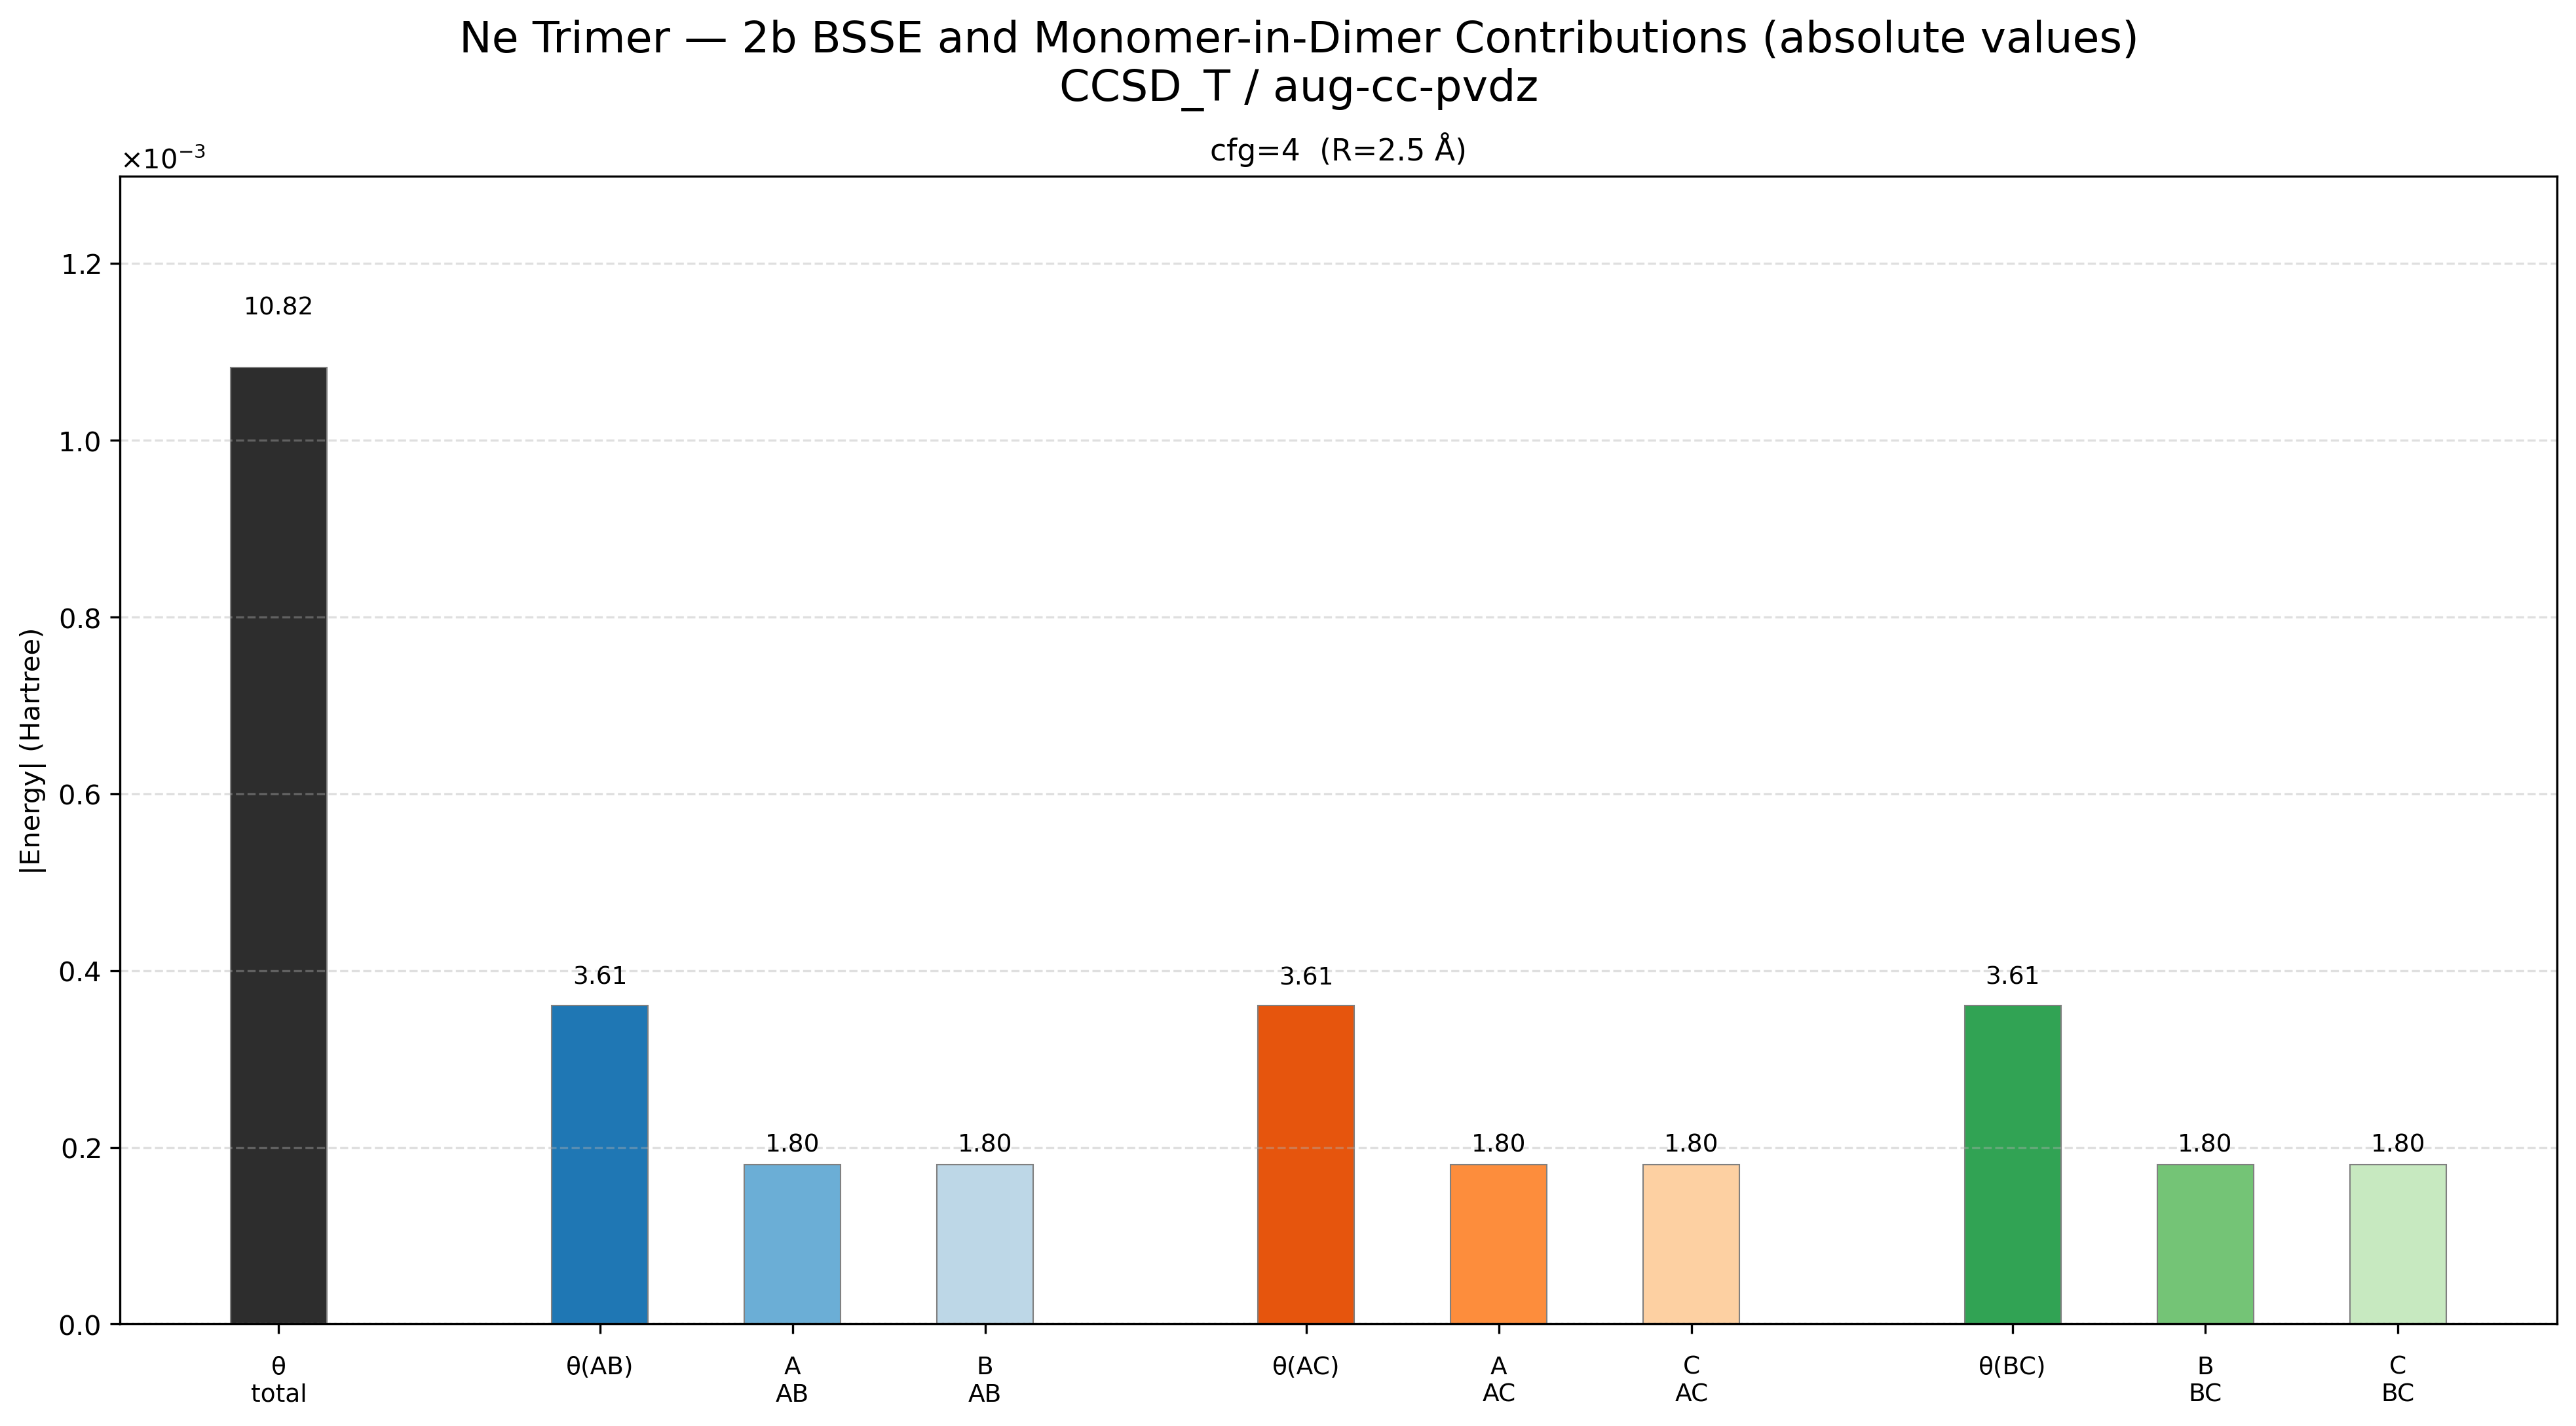
\includegraphics[width=1.0\textwidth]{figures/trimer/Ne_trimer/plot4_Ne_CCSD_T_aug-cc-pvdz_part5.png}
    \caption{FORM~II decomposition of the 2-body BSSE for the Ne
    trimer at $R = \SI{2.5}{\angstrom}$ (configuration~4),
    CCSD(T)/aug-cc-pVDZ. All values are absolute values in units
    of $10^{-3}$~Ha. Black bar: total 2-body BSSE
    $|\theta^{(2)}| = 10.82 \times 10^{-3}$~Ha. For each pair
    (AB, AC, BC) the pair total is $3.61 \times 10^{-3}$~Ha,
    and the two monomer-in-dimer-basis contributions are each
    $1.80 \times 10^{-3}$~Ha. All nine per-pair and
    per-monomer bars are identical, reflecting the perfect $C_{3v}$
    symmetry of the Ne trimer.}
    \label{fig:ne_trimer_plot4}
\end{figure}

At $R = \SI{2.5}{\angstrom}$ all three pair totals are equal:
$|\theta^{(2)}(\text{AB})| = |\theta^{(2)}(\text{AC})| =
|\theta^{(2)}(\text{BC})| = 3.61 \times 10^{-3}$~Ha. Within each
pair, the two monomer-in-dimer-basis contributions are also equal
($1.80 \times 10^{-3}$~Ha each), as required by the symmetry of the
equilateral triangle. The total 2-body BSSE is simply three times the
per-pair value: $3 \times 3.61 = 10.82 \times 10^{-3}$~Ha. This
complete equivalence of all bars in the decomposition is qualitatively
different from the \ce{H2O} trimer, where the AC pair was consistently
smaller than AB and BC.

% ----------------------------------------------------------------------
\subsection{Three-Body BSSE Decomposition at $R = \SI{2.5}{\angstrom}$}
% ----------------------------------------------------------------------

Figure~\ref{fig:ne_trimer_plot5} shows the FORM~II decomposition of
the 3-body BSSE at the same representative configuration.

\begin{figure}[!ht]
    \centering
    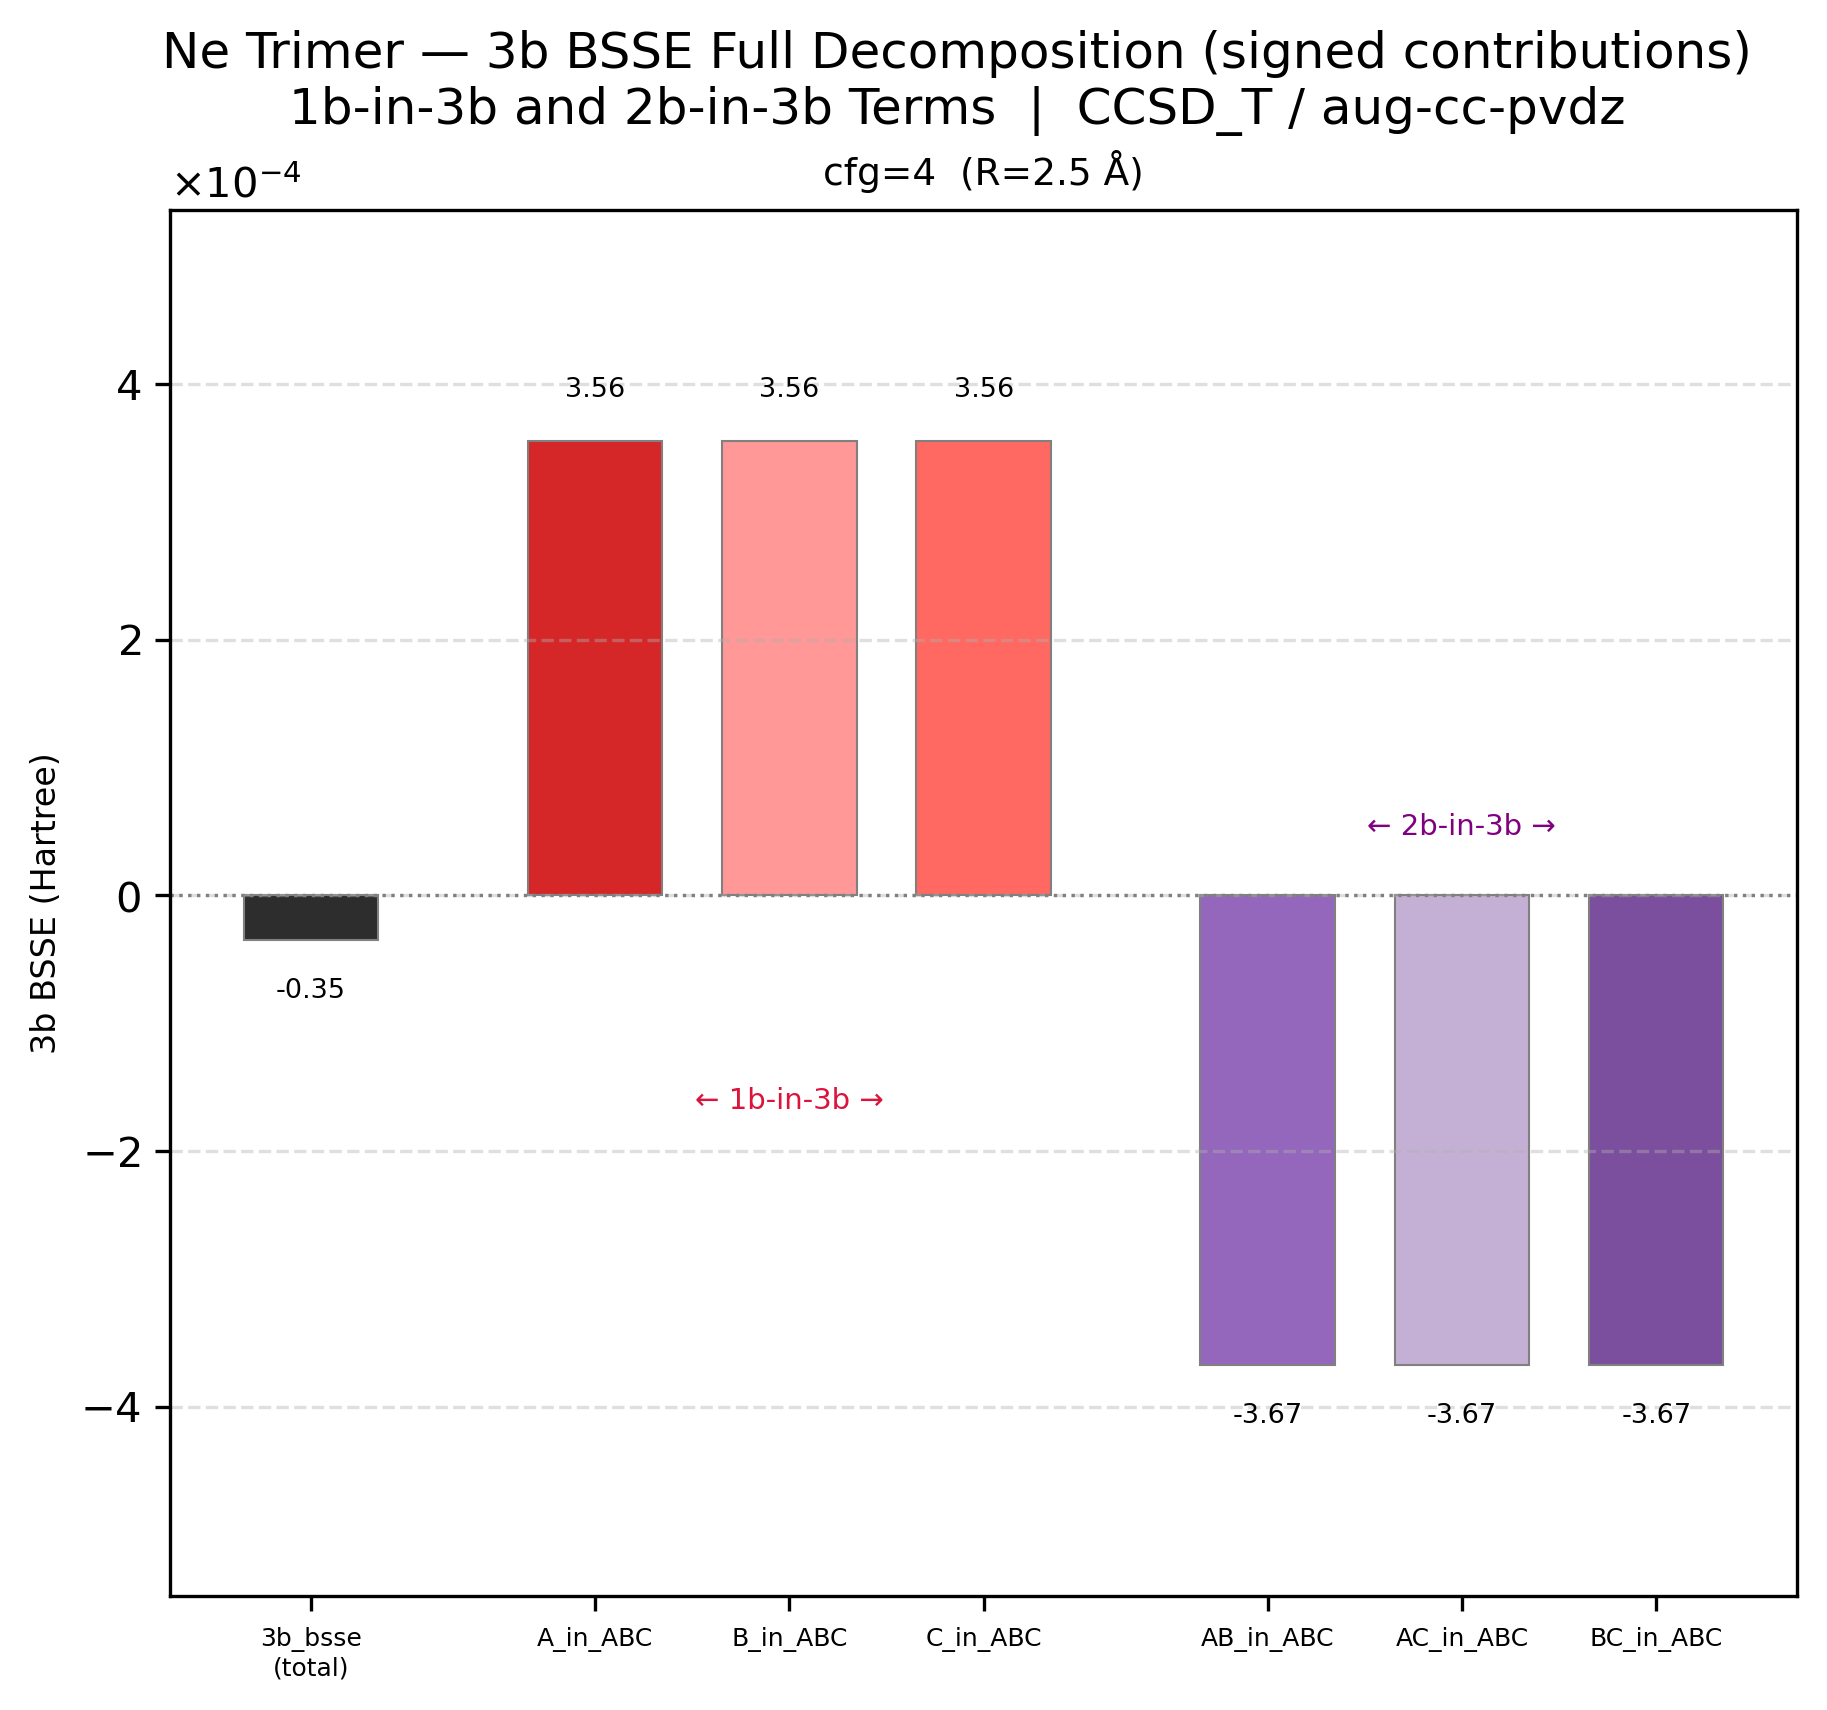
\includegraphics[width=1.0\textwidth]{figures/trimer/Ne_trimer/plot5_Ne_CCSD_T_aug-cc-pvdz_part5.png}
    \caption{FORM~II decomposition of the 3-body BSSE for the Ne
    trimer at $R = \SI{2.5}{\angstrom}$ (configuration~4),
    CCSD(T)/aug-cc-pVDZ. Signed contributions in units of
    $10^{-4}$~Ha. Black bar: total $\theta^{(3)} = -0.35 \times
    10^{-4}$~Ha. Red bars (positive): 1b-in-3b terms
    $\delta(\text{A in ABC}) = \delta(\text{B in ABC}) =
    \delta(\text{C in ABC}) = +3.56 \times 10^{-4}$~Ha.
    Purple bars (negative): 2b-in-3b terms
    $\delta(\text{AB in ABC}) = \delta(\text{AC in ABC}) =
    \delta(\text{BC in ABC}) = -3.67 \times 10^{-4}$~Ha.
    The two groups nearly cancel; the 2b-in-3b terms are slightly
    larger in magnitude, yielding a small negative net
    $\theta^{(3)}$ at this configuration.}
    \label{fig:ne_trimer_plot5}
\end{figure}

\clearpage

The 3-body BSSE $\theta^{(3)}$ again results from a near-cancellation
between the 1b-in-3b terms (positive, $+3.56 \times 10^{-4}$~Ha each)
and the 2b-in-3b terms (negative, $-3.67 \times 10^{-4}$~Ha each).
At $R = \SI{2.5}{\angstrom}$ the 2b-in-3b group is slightly larger
in magnitude, giving a net $\theta^{(3)} = -0.35 \times 10^{-4}$~Ha.
This configuration lies just below the sign-change distance: at $R
\geq \SI{2.75}{\angstrom}$ the 1b-in-3b terms come to dominate and
$\theta^{(3)}$ becomes positive at the MP2 and CCSD(T) levels. As
with the 2-body decomposition, all bars within each group are exactly
equal, a consequence of the perfect $C_{3v}$ symmetry.

% ----------------------------------------------------------------------
\subsection{Key Findings}
% ----------------------------------------------------------------------

\begin{finding_box}
\textbf{Perfect $C_{3v}$ symmetry makes all pair contributions
identical.}
Because the Ne trimer is an equilateral triangle of identical atoms,
$\theta^{(2)}(\text{AB}) = \theta^{(2)}(\text{AC}) =
\theta^{(2)}(\text{BC})$ at every configuration and every level of
theory. All FORM~II delta terms within each body-order group are also
equal. This is in contrast to the \ce{H2O} trimer, where the distinct
monomer orientations break the equivalence of the three pairs.
\end{finding_box}

\begin{finding_box}
\textbf{The 3-body BSSE changes sign with increasing Ne--Ne distance.}
At all three levels of theory the 3-body term $\theta^{(3)}$ is
negative at short range and becomes positive near $R =
\SI{2.75}{\angstrom}$. In all cases the magnitude of $\theta^{(3)}$
remains small relative to the 2-body total, and the 2-body term
dominates the total BSSE across the full range of distances sampled.
\end{finding_box}

\clearpage

% ======================================================================
\section{HF Trimer BSSE Results}
% ======================================================================

% ----------------------------------------------------------------------
\subsection{Total BSSE vs F--F Distance}
% ----------------------------------------------------------------------

Figure~\ref{fig:hf_trimer_plot1} shows the total BSSE as a function of
F--F distance $R$ for all three levels of theory.

\begin{figure}[!ht]
    \centering
    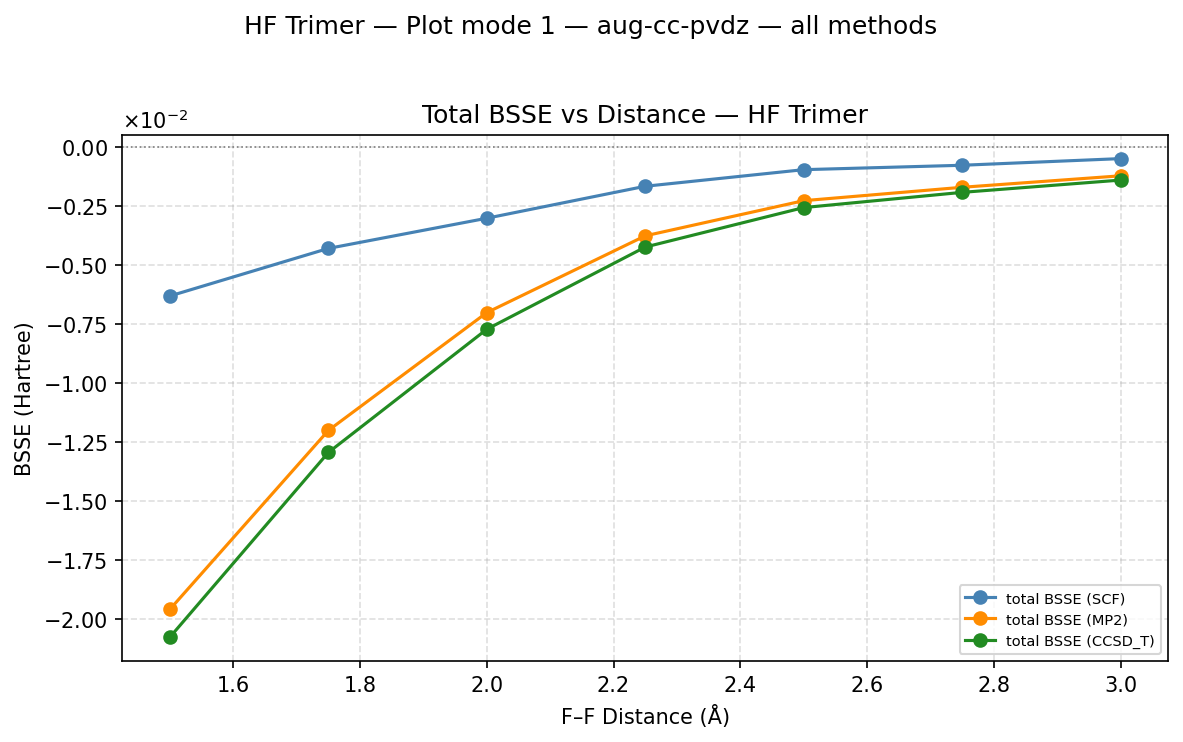
\includegraphics[width=1.0\textwidth]{figures/trimer/HF_trimer/plot1_HF_all_aug-cc-pvdz.png}
    \caption{Total BSSE vs F--F distance $R$ for the HF trimer at
    the aug-cc-pVDZ level. Blue circles: SCF; orange squares: MP2;
    green triangles: CCSD(T). All values are in Hartree. All three
    curves approach zero monotonically with increasing $R$. At the
    shortest distance ($R = \SI{1.5}{\angstrom}$) the total BSSE
    reaches approximately $-6.5 \times 10^{-3}$~Ha (SCF),
    $-1.95 \times 10^{-2}$~Ha (MP2), and $-2.1 \times 10^{-2}$~Ha
    (CCSD(T)). Unlike the Ne and \ce{H2O} trimers, the MP2 and
    CCSD(T) curves are significantly larger in magnitude than the
    SCF contribution across the full range, reflecting the strong
    hydrogen-bonding network in the HF cluster.}
    \label{fig:hf_trimer_plot1}
\end{figure}

All three curves are negative and approach zero monotonically with
increasing $R$. The BSSE magnitude is substantially larger for the
HF trimer than for either the Ne or \ce{H2O} trimers at comparable
distances, consistent with the larger basis sets required to describe
the fluorine lone pairs and the H-bond donor--acceptor interactions.
The MP2 and CCSD(T) values are approximately three times larger in
magnitude than the SCF contribution at short range, a significantly
greater correlated enhancement than observed for the other two
molecules.

% ----------------------------------------------------------------------
\subsection{Two-Body and Three-Body Decomposition}
% ----------------------------------------------------------------------

Figure~\ref{fig:hf_trimer_plot2} separates the total BSSE into its
two-body ($\theta^{(2)}$) and three-body ($\theta^{(3)}$) components
for each level of theory.

\begin{figure}[!ht]
    \centering
    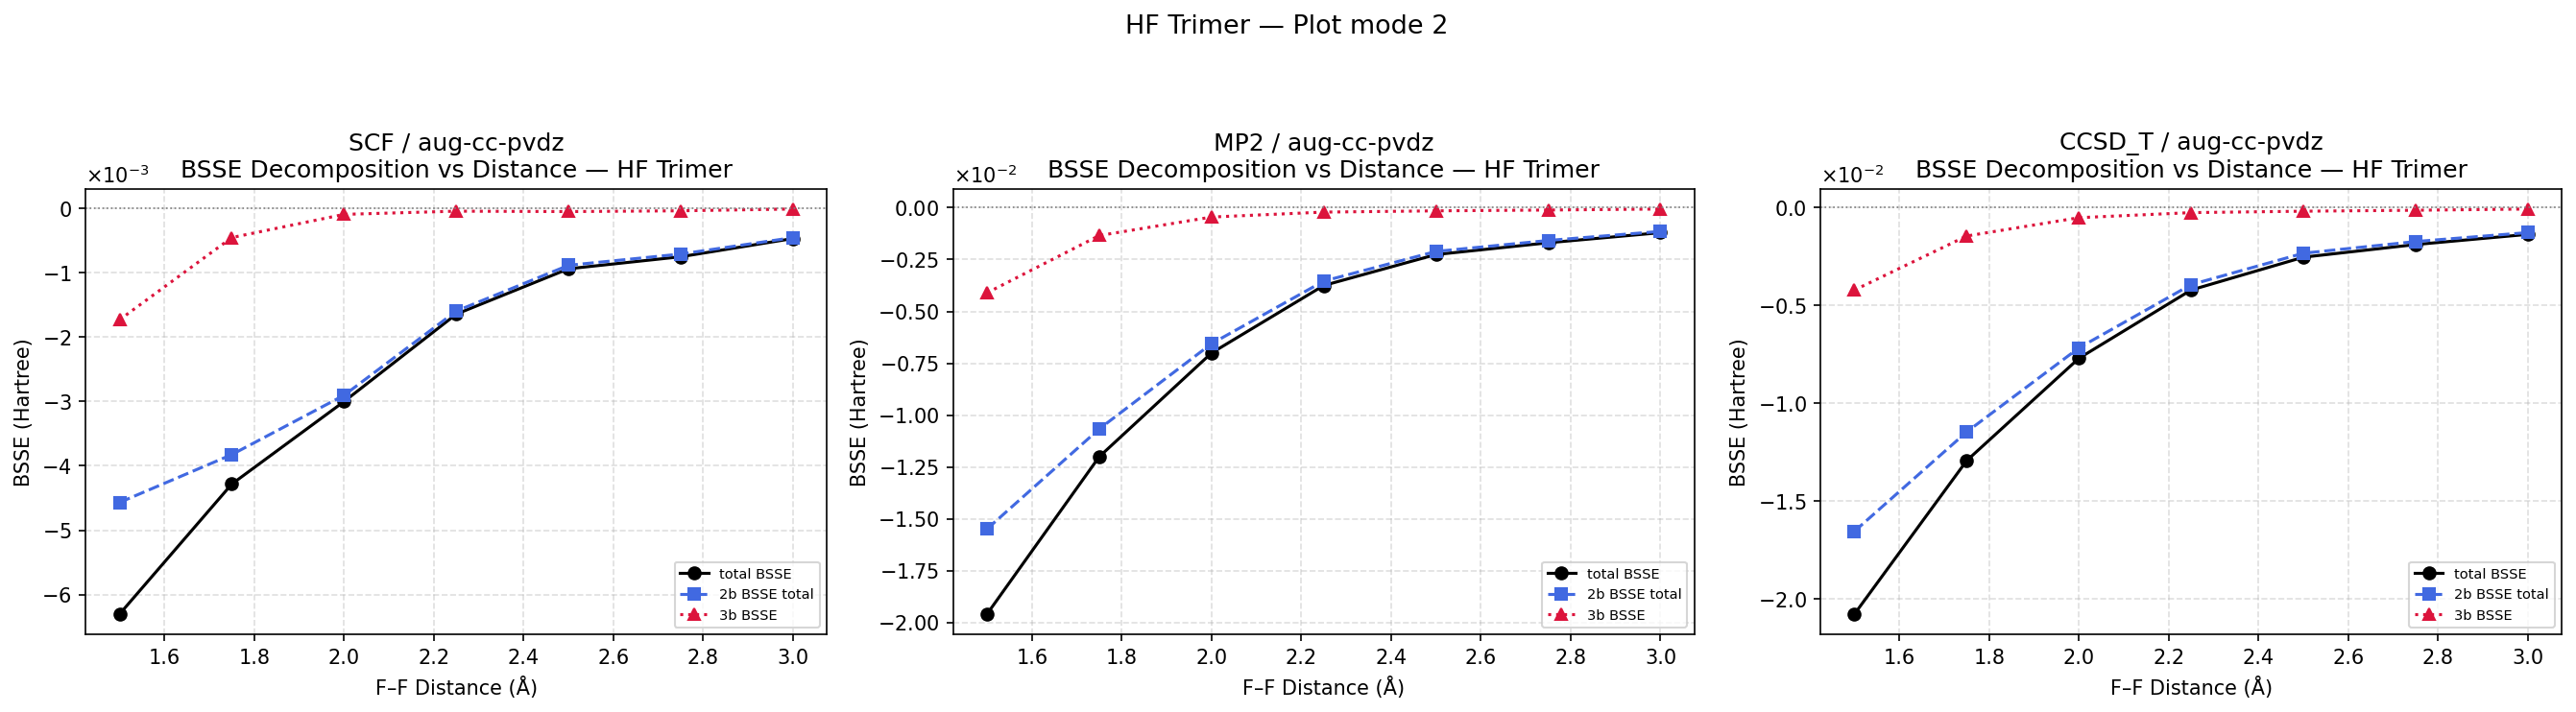
\includegraphics[width=0.7\textwidth]{figures/trimer/HF_trimer/plot2_HF_all_aug-cc-pvdz.png}
    \caption{BSSE body-order decomposition vs F--F distance $R$ for
    the HF trimer at the aug-cc-pVDZ level. Each panel corresponds to
    one level of theory (SCF, MP2, CCSD(T)). Black circles: total
    BSSE; blue dashed squares: 2-body total ($\theta^{(2)}$); red
    dashed triangles: 3-body term ($\theta^{(3)}$). Unlike the Ne and
    \ce{H2O} trimers, a clear gap exists between the total BSSE and
    the 2-body total at all methods and distances, indicating a
    significant 3-body contribution. The 3-body term $\theta^{(3)}$
    is negative at all distances and all levels of theory --- the same
    sign as the 2-body total --- and does not change sign across the
    range of $R$ sampled.}
    \label{fig:hf_trimer_plot2}
\end{figure}

In contrast to the Ne and \ce{H2O} trimers, the total BSSE and the
2-body total are visibly distinct in all three panels. The 3-body
contribution $\theta^{(3)}$ is negative at all distances and all
levels of theory, carrying the same sign as the 2-body total and
adding constructively to it. This behavior --- a large, negative
$\theta^{(3)}$ that never changes sign --- distinguishes the HF
trimer from both Ne (which shows a sign change) and \ce{H2O} (where
$\theta^{(3)}$ is positive and near-negligible).

% TODO: pending PI discussion — physical interpretation of the sign
% and magnitude of theta^(3) in the HF trimer relative to Ne and H2O.

% ----------------------------------------------------------------------
\subsection{Per-Pair Two-Body BSSE}
% ----------------------------------------------------------------------

Figure~\ref{fig:hf_trimer_plot3} resolves the 2-body BSSE into
contributions from each of the three monomer pairs: AB, AC, and BC.

\begin{figure}[!ht]
    \centering
    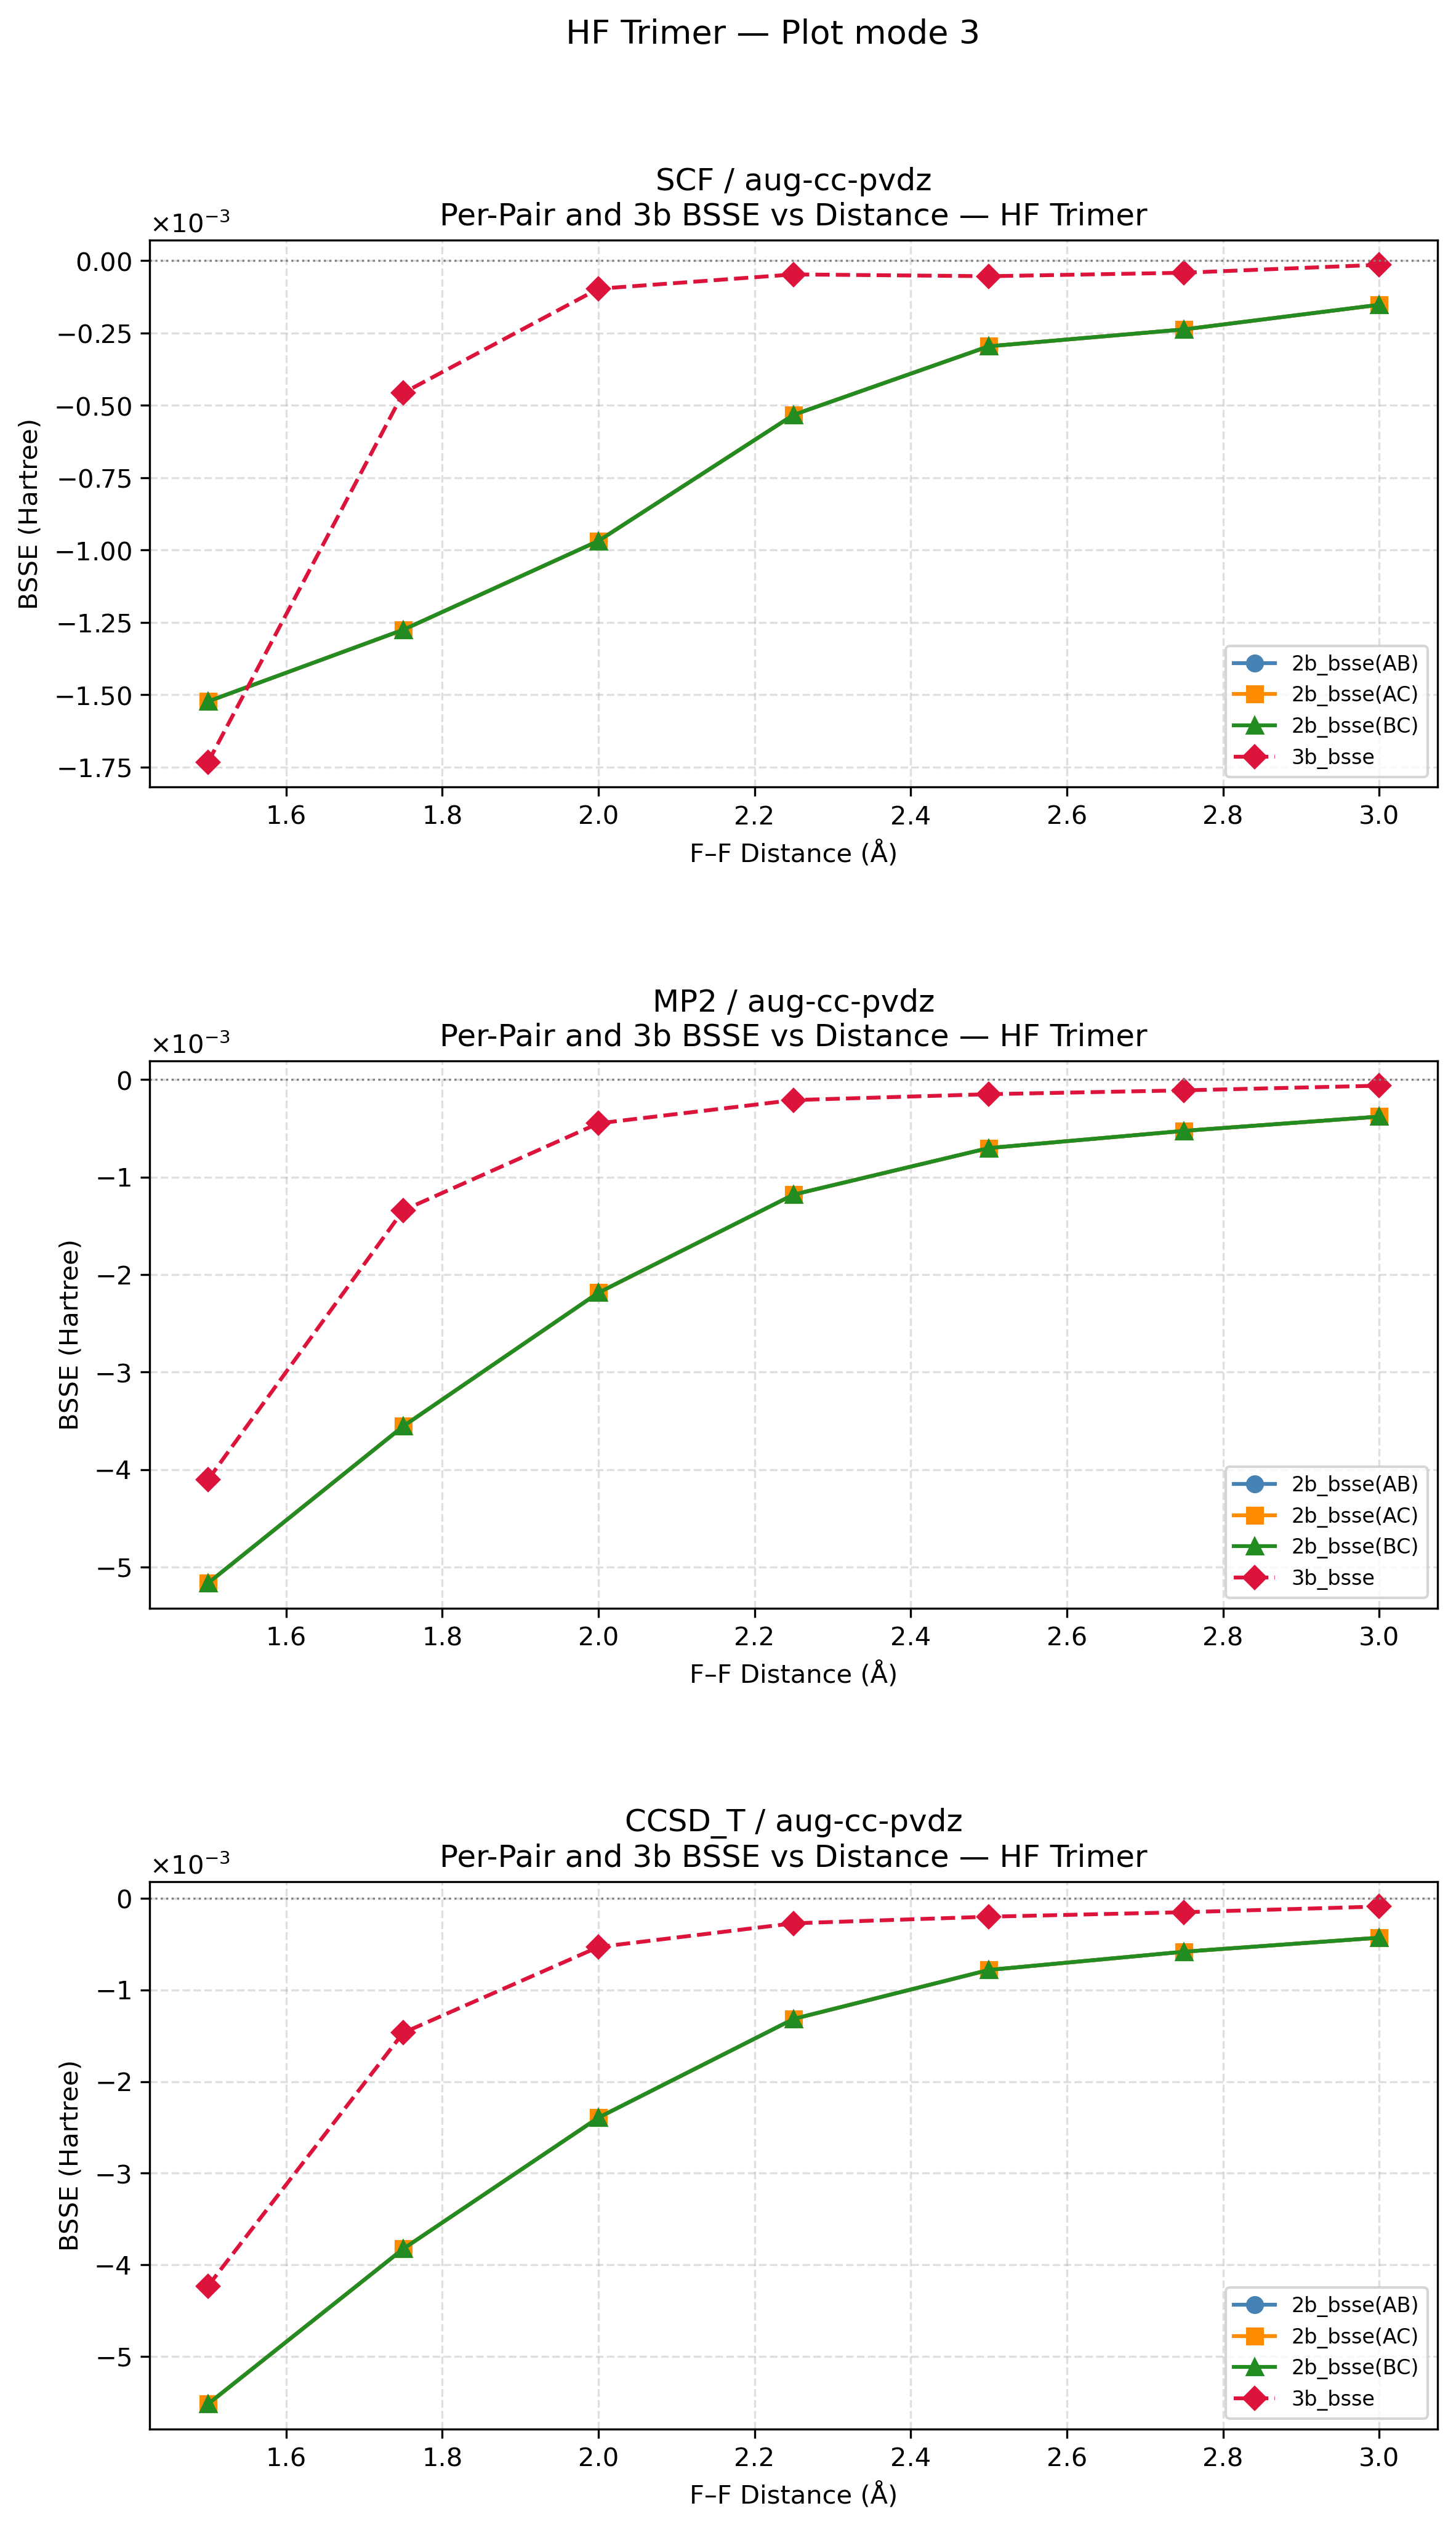
\includegraphics[width=0.7\textwidth]{figures/trimer/HF_trimer/plot3_HF_all_aug-cc-pvdz.png}
    \caption{Per-pair 2-body and 3-body BSSE vs F--F distance $R$
    for the HF trimer at the aug-cc-pVDZ level. Each panel corresponds
    to one level of theory. Blue circles: $\theta^{(2)}$(AB); orange
    squares: $\theta^{(2)}$(AC); green triangles: $\theta^{(2)}$(BC);
    red dashed diamonds: $\theta^{(3)}$. The three pair contributions
    are exactly equal at every distance and every level of theory:
    $\theta^{(2)}(\text{AB}) = \theta^{(2)}(\text{AC}) =
    \theta^{(2)}(\text{BC})$ at all $R$. The 3-body term is negative
    and of comparable magnitude to the individual pair contributions
    at short range.}
    \label{fig:hf_trimer_plot3}
\end{figure}

As with the Ne trimer, the three pair contributions are numerically
identical at every configuration and every level of theory, and the
three symbols lie exactly on top of one another in
Figure~\ref{fig:hf_trimer_plot3}. This reflects the equilateral
arrangement of the fluorine atoms and the equivalence of the three
HF monomers. A notable feature of the HF trimer is the magnitude of
$\theta^{(3)}$ relative to the per-pair contributions: at short range
the 3-body term is comparable in magnitude to a single pair
contribution, a much larger relative 3-body effect than seen in
either Ne or \ce{H2O}.

% TODO: pending PI discussion — physical interpretation of large
% relative 3-body contribution at short range in the HF trimer.

\clearpage

% ----------------------------------------------------------------------
\subsection{Two-Body BSSE Decomposition at $R = \SI{2.25}{\angstrom}$}
% ----------------------------------------------------------------------

Figure~\ref{fig:hf_trimer_plot4} shows the FORM~II decomposition of
the 2-body BSSE at the representative configuration $R =
\SI{2.25}{\angstrom}$ (configuration~3) at the CCSD(T) level.

\begin{figure}[!ht]
    \centering
    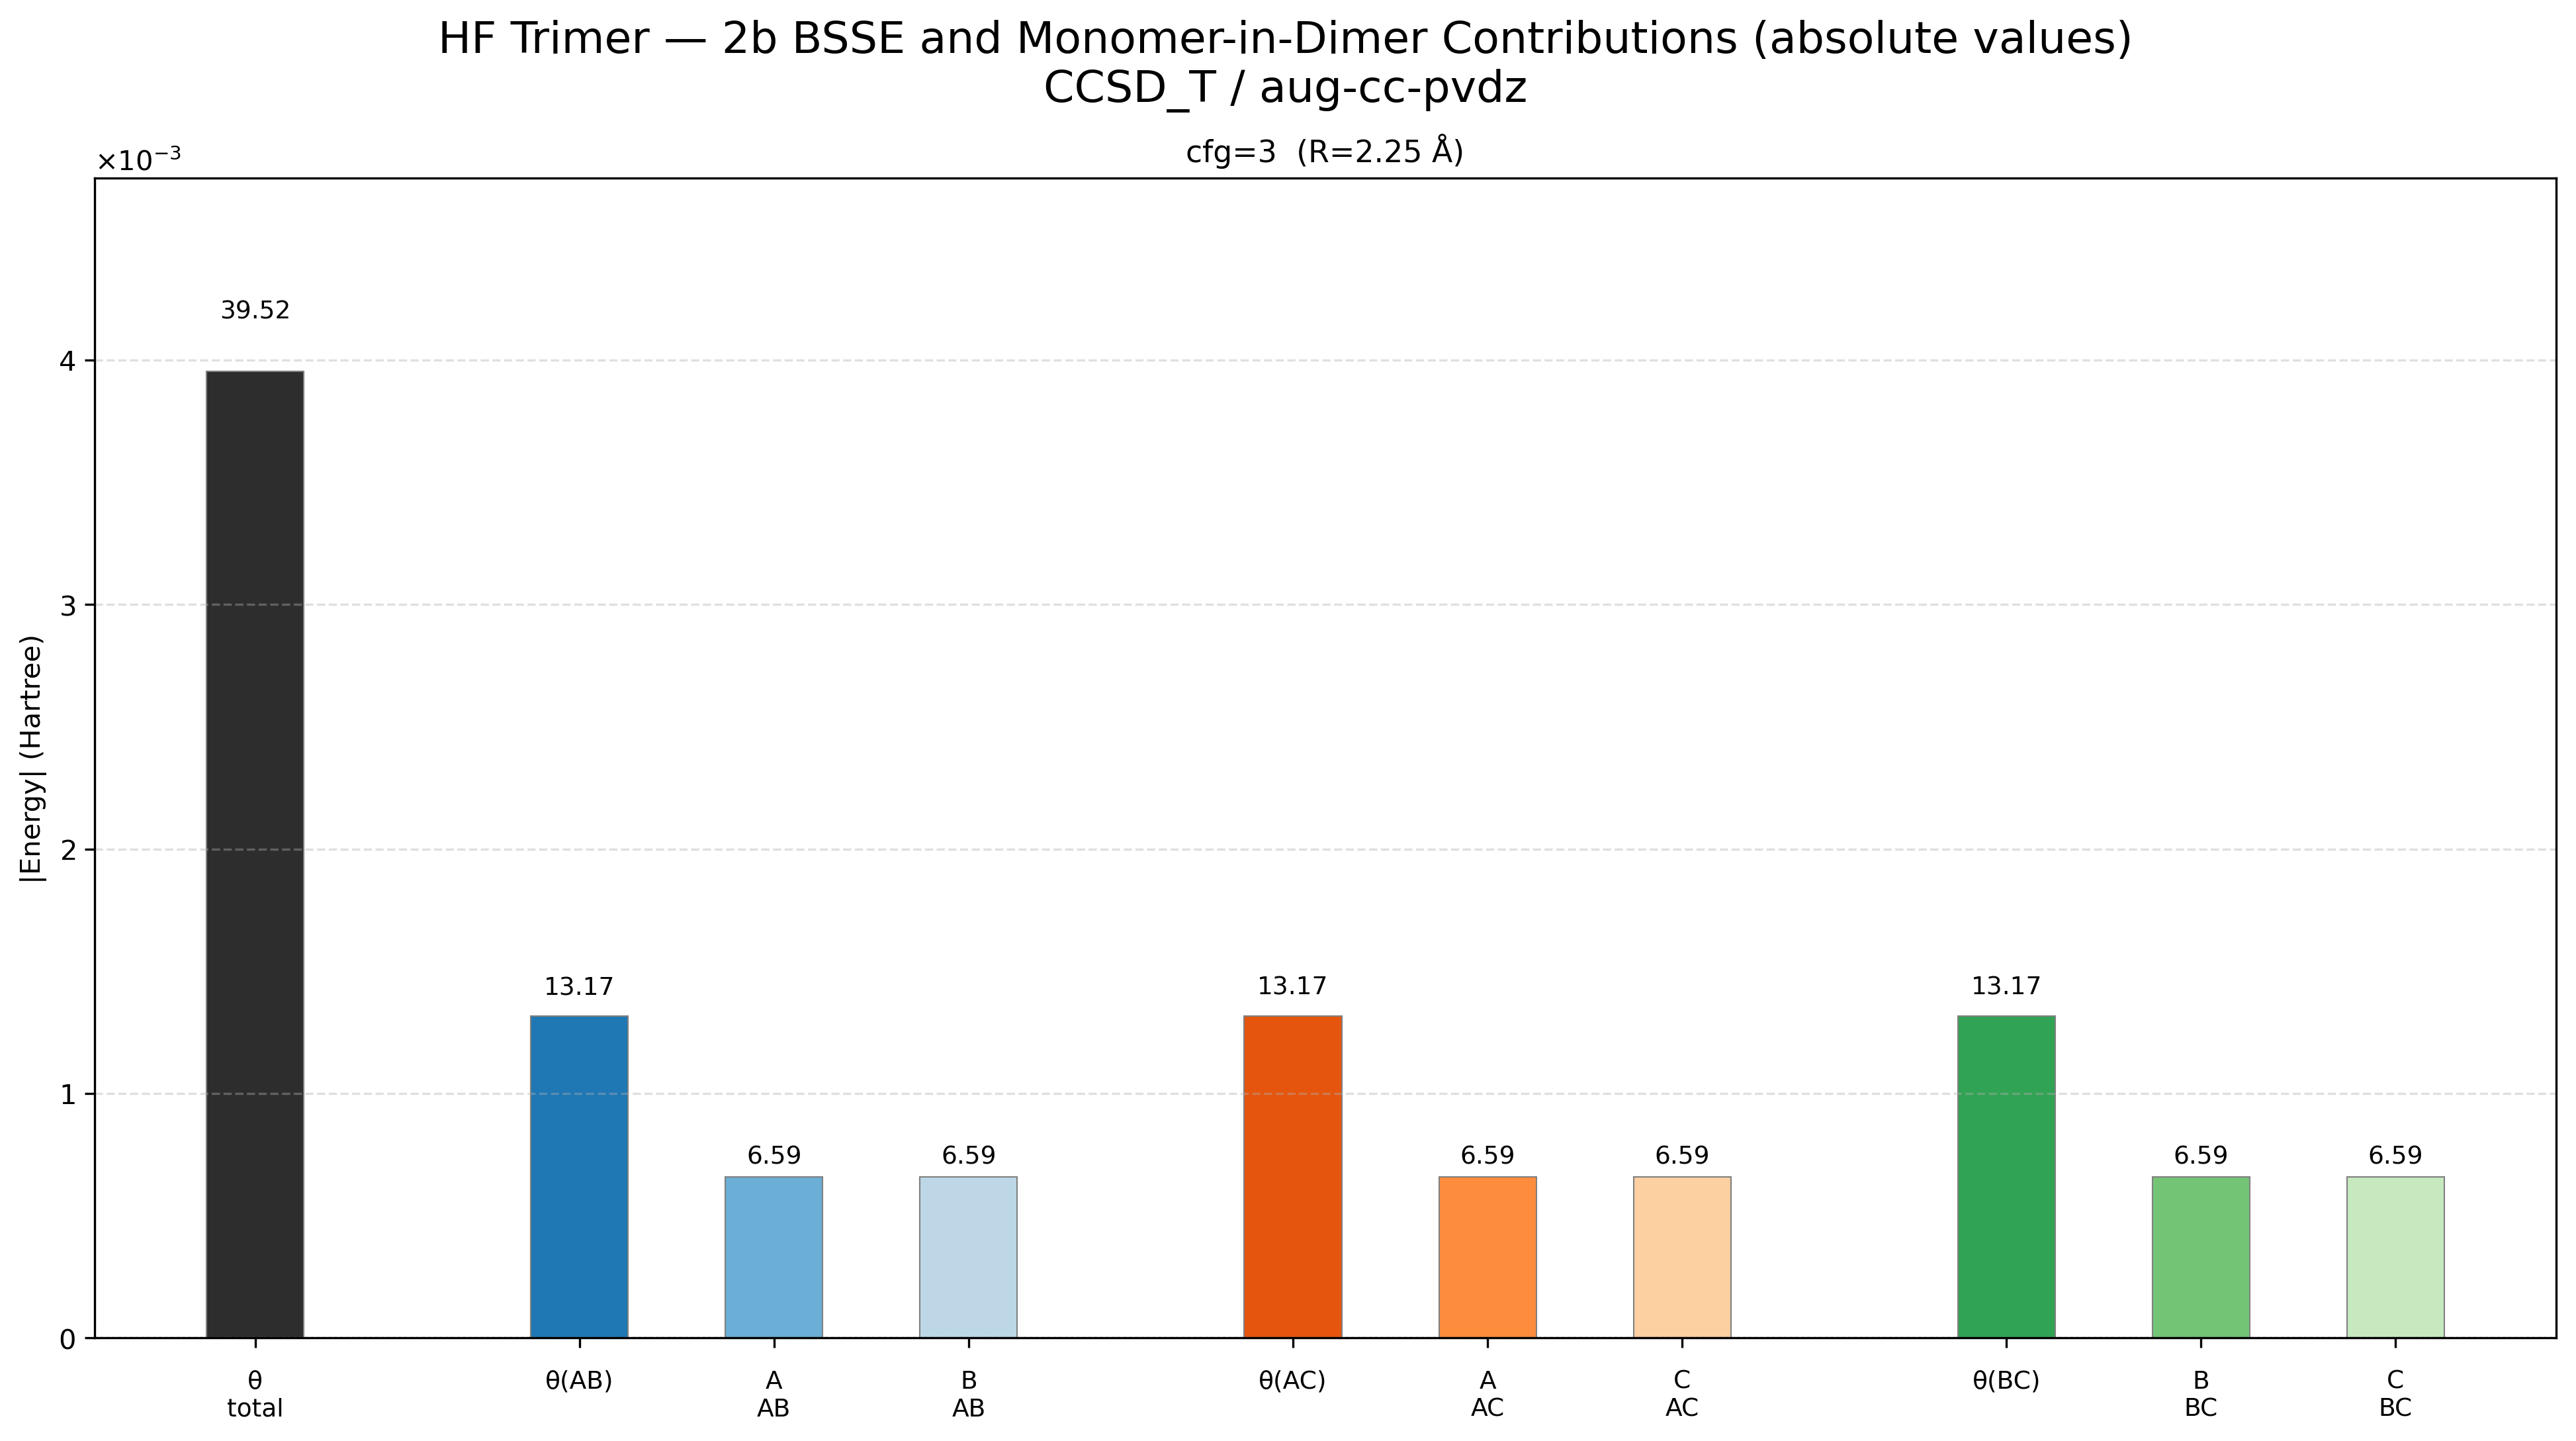
\includegraphics[width=1.0\textwidth]{figures/trimer/HF_trimer/plot4_HF_CCSD_T_aug-cc-pvdz_part4.png}
    \caption{FORM~II decomposition of the 2-body BSSE for the HF
    trimer at $R = \SI{2.25}{\angstrom}$ (configuration~3),
    CCSD(T)/aug-cc-pVDZ. All values are absolute values in units
    of $10^{-3}$~Ha. Black bar: total 2-body BSSE
    $|\theta^{(2)}| = 39.52 \times 10^{-3}$~Ha. For each pair
    (AB, AC, BC) the pair total is $13.17 \times 10^{-3}$~Ha,
    and the two monomer-in-dimer-basis contributions are each
    $6.59 \times 10^{-3}$~Ha. All nine per-pair and per-monomer
    bars are identical, reflecting the equilateral symmetry of
    the HF trimer at this geometry.}
    \label{fig:hf_trimer_plot4}
\end{figure}

At $R = \SI{2.25}{\angstrom}$ all three pair totals are equal:
$|\theta^{(2)}(\text{AB})| = |\theta^{(2)}(\text{AC})| =
|\theta^{(2)}(\text{BC})| = 13.17 \times 10^{-3}$~Ha, and within
each pair the two monomer-in-dimer-basis contributions are also equal
($6.59 \times 10^{-3}$~Ha each). The total 2-body BSSE is three times
the per-pair value: $3 \times 13.17 = 39.52 \times 10^{-3}$~Ha.
Comparing to the Ne trimer at its representative configuration
($10.82 \times 10^{-3}$~Ha), the HF 2-body BSSE is approximately
four times larger at this distance, reflecting the much larger basis
set requirements of the fluorine and hydrogen atoms in a
hydrogen-bonding environment.

% ----------------------------------------------------------------------
\subsection{Three-Body BSSE Decomposition at $R = \SI{2.25}{\angstrom}$}
% ----------------------------------------------------------------------

Figure~\ref{fig:hf_trimer_plot5} shows the FORM~II decomposition of
the 3-body BSSE at the same representative configuration.

\begin{figure}[!ht]
    \centering
    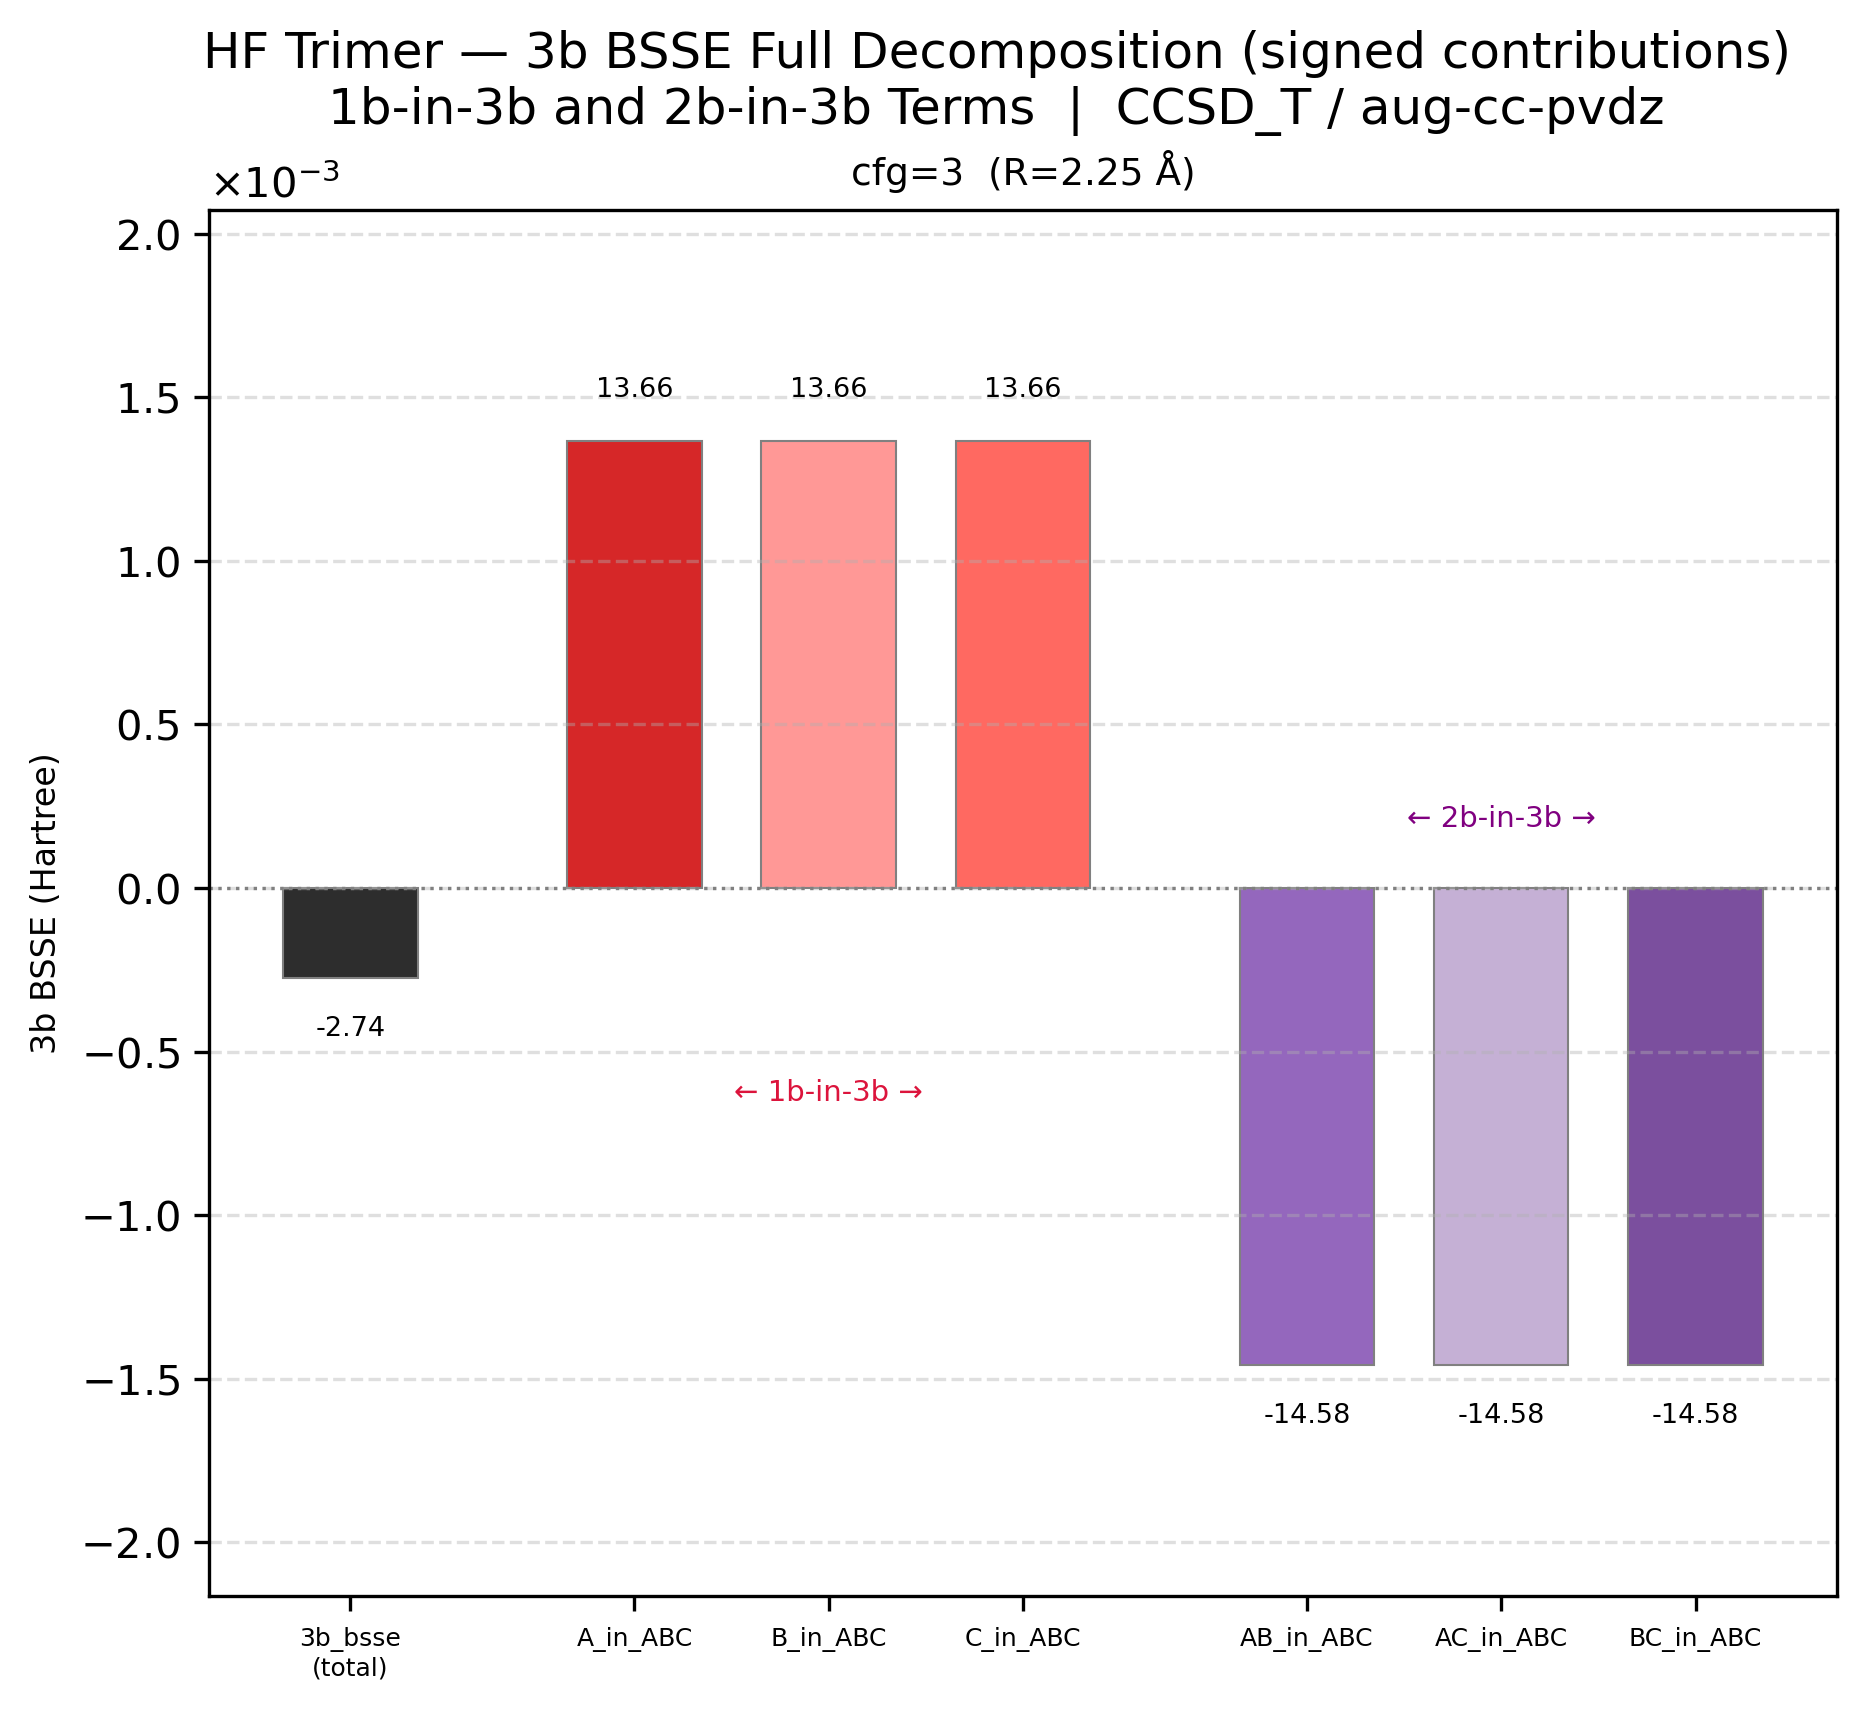
\includegraphics[width=1.0\textwidth]{figures/trimer/HF_trimer/plot5_HF_CCSD_T_aug-cc-pvdz_part4.png}
    \caption{FORM~II decomposition of the 3-body BSSE for the HF
    trimer at $R = \SI{2.25}{\angstrom}$ (configuration~3),
    CCSD(T)/aug-cc-pVDZ. Signed contributions in units of
    $10^{-3}$~Ha. Black bar: total $\theta^{(3)} = -2.74 \times
    10^{-3}$~Ha. Red bars (positive): 1b-in-3b terms
    $\delta(\text{A in ABC}) = \delta(\text{B in ABC}) =
    \delta(\text{C in ABC}) = +13.66 \times 10^{-3}$~Ha.
    Purple bars (negative): 2b-in-3b terms
    $\delta(\text{AB in ABC}) = \delta(\text{AC in ABC}) =
    \delta(\text{BC in ABC}) = -14.58 \times 10^{-3}$~Ha.
    The 2b-in-3b group dominates over the 1b-in-3b group, yielding
    a net negative $\theta^{(3)}$. Note the $\times 10^{-3}$~Ha
    scale --- an order of magnitude larger than the corresponding
    Ne trimer decomposition.}
    \label{fig:hf_trimer_plot5}
\end{figure}

\clearpage

The structure of the 3-body BSSE decomposition for HF mirrors the
pattern seen for Ne and \ce{H2O}: a near-cancellation between the
positive 1b-in-3b terms and the negative 2b-in-3b terms. However,
for HF the 2b-in-3b group dominates more substantially, with each
term ($-14.58 \times 10^{-3}$~Ha) exceeding the corresponding
1b-in-3b term ($+13.66 \times 10^{-3}$~Ha) by approximately 7\%.
This imbalance yields a net $\theta^{(3)} = -2.74 \times 10^{-3}$~Ha,
which is negative at this configuration and at all configurations
sampled (Figure~\ref{fig:hf_trimer_plot2}). All bars within each
group are exactly equal, confirming the equilateral symmetry of the
cluster. The overall scale --- $10^{-3}$~Ha versus $10^{-4}$~Ha for
Ne --- underscores the much larger 3-body BSSE in the HF trimer.

% ----------------------------------------------------------------------
\subsection{Key Findings}
% ----------------------------------------------------------------------

\begin{finding_box}
\textbf{The 3-body BSSE is large and negative at all HF trimer
configurations.}
Unlike the Ne trimer (where $\theta^{(3)}$ changes sign with $R$) and
the \ce{H2O} trimer (where $\theta^{(3)}$ is positive and
near-negligible), the HF trimer shows a large negative $\theta^{(3)}$
at every F--F distance and every level of theory sampled. The 3-body
contribution adds constructively to the 2-body total, making the total
BSSE significantly larger than the 2-body term alone. At the shortest
distance ($R = \SI{1.5}{\angstrom}$) the $|\theta^{(3)}/\theta^{(2)}|$
ratio reaches approximately 25\% at the CCSD(T) level.
\end{finding_box}

\begin{finding_box}
\textbf{The FORM~II decomposition shows a persistent 2b-in-3b
dominance.}
At all configurations the 3-body BSSE arises from a near-cancellation
between the positive 1b-in-3b and negative 2b-in-3b FORM~II delta
terms, with the 2b-in-3b group always larger in magnitude. At the
representative configuration ($R = \SI{2.25}{\angstrom}$, CCSD(T))
each 2b-in-3b term is $-14.58 \times 10^{-3}$~Ha and each 1b-in-3b
term is $+13.66 \times 10^{-3}$~Ha, yielding a net
$\theta^{(3)} = -2.74 \times 10^{-3}$~Ha. This contrasts with the
Ne trimer at longer range, where the 1b-in-3b group comes to dominate
and $\theta^{(3)}$ turns positive.
% TODO: pending PI discussion — physical interpretation of persistent
% 2b-in-3b dominance and sign difference relative to Ne trimer.
\end{finding_box}

\clearpage